% 第 7 章 欧几里得与酉向量空间 (Euklidische und unitäre Vektorräume)
\chapter{欧几里得与酉向量空间}\index{oujilidexiangliangkongjian@欧几里得向量空间(euklidischer Vektorraum)}\index{youxiangliangkongjian@酉向量空间(unitärer Vektorraum)}

\section*{预备说明}

在第 1 章的预备说明中我们曾经考虑过, 用何种方式才能把 $\mathbb{R}$-向量空间 $\mathbb{R}^2$ 解释为直观平面的模型.若想在这个模型中正确地反映距离,从而最终也正确地反映角度, 就必须给模型配备一个距离函数.例如在 $\mathbb{R}^2$ 中, 两点 $P_1 = (x_1, y_1)$, $P_2 = (x_2, y_2)$ 之间的通常欧几里得距离由

\[
d(P_1, P_2) = \sqrt{(x_1 - x_2)^2 + (y_1 - y_2)^2}
\]

给出, 而向量 $\overrightarrow{0P_1}$ 的长度或模长由

\[
|\overrightarrow{0P_1}| := |P_1| := \sqrt{x_1^2 + y_1^2}
\]

给出.

由此借助

\[
\langle P_1, P_2 \rangle := \frac{1}{2}\bigl(|P_1 + P_2|^2 - |P_1|^2 - |P_2|^2\bigr) = x_1 x_2 + y_1 y_2
\]

得到一个含两个变量的函数, 即所谓的\emph{对称双线性形式}(\textup{symmetrische Bilinearform})\index{duichenshuangxianxingxingshi@对称双线性形式(symmetrische Bilinearform)}, 在我们这里甚至是数量积, 它满足 $|P_1| = \sqrt{\langle P_1, P_1 \rangle}$.下面的观察可以作为这样一个数量积也能刻画角度的佐证: 数量积 $\langle P_1, P_2 \rangle$ 消失, 当且仅当 $|P_1 + P_2|^2 = |P_1|^2 + |P_2|^2$ 成立.对非平凡的 $P_1$, $P_2$, 依据\emph{勾股定理}(\textup{Pythagoras, Satz von})\index{gougudingli@勾股定理(Pythagoras, Satz von)}的逆定理, 这等价于向量 $\overrightarrow{0P_1}$ 与 $\overrightarrow{0P_2}$ 互相\emph{垂直}(\textup{senkrecht})\index{chuizhi@垂直(senkrecht)}:

\begin{center}
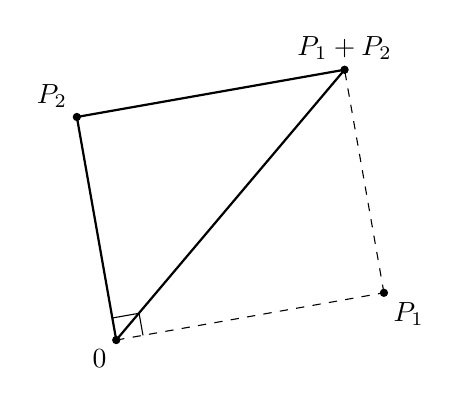
\begin{tikzpicture}[>=latex]
  \coordinate (O)  at (0,0);
  \coordinate (P1) at (3.4,0.6);
  \coordinate (P2) at (-0.5,2.833);
  \coordinate (P)  at (2.9,3.433);
  
  \draw[thick] (O) -- (P2);
  \draw[thick] (P2) -- (P);
  \draw[thick] (O) -- (P);
  
  \draw[dashed] (O) -- (P1);
  \draw[dashed] (P1) -- (P);
  
  % 直角标记
  \draw (0.34,0.06) -- (0.29,0.34) -- (-0.05,0.28);
  
  \fill (O)  circle (1.5pt) node[below left]{$0$};
  \fill (P1) circle (1.5pt) node[below right]{$P_1$};
  \fill (P2) circle (1.5pt) node[above left]{$P_2$};
  \fill (P)  circle (1.5pt) node[above]{$P_1 + P_2$};
\end{tikzpicture}
\end{center}

本章的主题是研究有限维 $\mathbb{R}$-和 $\mathbb{C}$-向量空间 $V$, 它们配备有由数量积 $\langle \cdot, \cdot \rangle \colon V \times V \longrightarrow K$ 给出的距离函数, 其中对 $K$ 要分别代入所考虑的基础域 $\mathbb{R}$ 或 $\mathbb{C}$.此时我们称为欧几里得或\emph{酉向量空间}(\textup{unitärer Vektorraum})\index{youxiangliangkongjian@酉向量空间(unitärer Vektorraum)}.最重要的例子是带有数量积 $\langle x, y \rangle = \sum_{i = 1}^{n} x_i \overline{y}_i$ 的向量空间 $K^n$, 其中 $\overline{y}_i$ 分别表示与 $y_i$ 共轭的复数.每个数量积都满足\emph{柯西-施瓦茨不等式}(\textup{Schwarz'sche Ungleichung})\index{kexishiwacibudengshi@柯西-施瓦茨不等式(Schwarz'sche Ungleichung)} $|\langle x, y \rangle| \leq |x| \, |y|$($x, y \in V$), 由它特别还可得到\emph{三角不等式}(\textup{Dreiecksungleichung})\index{sanjiaobudengshi@三角不等式(Dreiecksungleichung)} $|x + y| \leq |x| + |y|$.

作为基本工具, 我们将讨论以 E.~施密特(E. Schmidt)命名的\emph{正交规范化方法}(\textup{Schmidt'sches Orthonormalisierungsverfahren})\index{zhengjiaoguifanhuafangfa@正交规范化方法(Schmidt'sches Orthonormalisierungsverfahren)}.它允许我们从一个任意的基 $x_1, \ldots, x_n$ 出发, 通过逐次改变诸 $x_i$, 构造出一个所谓的\emph{标准正交基}(\textup{Orthonormalbasis})\index{biaozhunzhengjiaoji@标准正交基(Orthonormalbasis)} $e_1, \ldots, e_n$, 它满足 $|e_i| = 1$ 对一切 $i$ 以及 $\langle e_i, e_j \rangle = 0$ 对一切 $i \neq j$ 成立.这样的标准正交基于是可以看作 $V$ 中的一个直角坐标系.此外, 由于双线性性, $V$ 的数量积可以很容易地借助 $V$ 的一个标准正交基重新构造出来, 因此一个带有数量积形式的距离函数的向量空间 $V$, 只要知道了 $V$ 中的一个标准\emph{正交基}(\textup{Orthogonalbasis})\index{zhengjiaoji@正交基(Orthogonalbasis)}, 就已经被完全确定.

在第 6 章中, 我们研究了有限维向量空间 $V$(系数在任意域 $K$ 中)上自同态 $f \colon V \longrightarrow V$ 的标准形.例如, 若 $f$ 关于 $V$ 的某个基 $X$ 由矩阵 $A_{f, X, X}$ 给出, 那么问题就在于寻找一个基变换矩阵 $A_{\id, X', X}$, 使得矩阵

\[
A_{f, X', X'} = (A_{\id, X', X})^{-1} \cdot A_{f, X, X} \cdot A_{\id, X', X}
\]

具有尽可能"简单"的形式.换言之, 我们借助标准形理论确定了 $K^{n \times n}$ 中矩阵的相似类, 其中两个矩阵 $A, B \in K^{n \times n}$ 称为相似的, 如果存在可逆矩阵 $S \in \mathrm{Gl}(n, K)$ 使得 $B = S^{-1} \cdot A \cdot S$ 成立.

现在我们想也在欧几里得与酉向量空间 $V$ 的框架内处理一个类似的问题.不过这里我们必须把 $V$ 上的距离函数一并考虑在内.因此我们只允许这样的基变换矩阵 $A_{\id, X', X}$, 它们保持长度, 从而定义出标准正交基 $X$ 与 $X'$ 之间的变换.后者恰好发生在

\[
(A_{\id, X', X})^{-1} = (A_{\id, X', X})^* := \overline{A_{\id, X', X}}^{t}
\]

成立的情形, 其中对矩阵 $A = (\alpha_{ij}) \in K^{n \times n}$, 相应的复\emph{共轭矩阵}(\textup{konjugierte Matrix})\index{gongejuzhen@共轭矩阵(konjugierte Matrix)} $\overline{A}$ 由 $\overline{A} = (\overline{\alpha}_{ij})$ 给出; 具有上述性质的矩阵 $S = A_{\id, X', X}$ 称为\emph{正交}(\textup{orthogonal})\index{zhengjiao@正交(orthogonal)}的(当 $K = \mathbb{R}$)或酉的(当 $K = \mathbb{C}$).由这样的矩阵定义的 $K^{n \times n}$ 中矩阵的等价关系, 因而比第 6 章所考虑的一般矩阵等价关系要严密得多.所以对标准形问题, 把注意力限制在 $K^{n \times n}$ 的某些子类上是合理的.我们在这里本质上只考虑\emph{对称矩阵}(\textup{symmetrische Matrix})\index{duichenjuzhen@对称矩阵(symmetrische Matrix)}或\emph{埃尔米特矩阵}(\textup{hermitesche Matrix})\index{aiermitejuzhen@埃尔米特矩阵(hermitesche Matrix)}, 即满足 $A = A^*$ 的矩阵 $A \in K^{n \times n}$; 关于标准正交基, 它们恰好代表所谓的自\emph{伴随自同态}(\textup{adjungierter Endomorphismus})\index{bansuizitongtai@伴随自同态(adjungierter Endomorphismus)} $f \colon V \longrightarrow V$, 后者满足关系 $\langle f(x), y \rangle = \langle x, f(y) \rangle$($x, y \in V$).不过此时我们能够证明一个令人惊讶的事实: 这样的矩阵在借助正交或\emph{酉矩阵}(\textup{unitäre Matrix})\index{youjuzhen@酉矩阵(unitäre Matrix)}的,更严格的等价意义下, 总是等价于一个实对角矩阵.

在上述分类问题中获得的成果, 也可以富有成效地应用于有限维 $K$-向量空间 $V$ 上对称\emph{双线性形式}(\textup{Bilinearform})\index{shuangxianxingxingshi@双线性形式(Bilinearform)}(当 $K = \mathbb{R}$)或\emph{埃尔米特形式}(\textup{hermitesche Form; HF})\index{aiermitexingshi@埃尔米特形式(hermitesche Form; HF)}(当 $K = \mathbb{C}$)的分类, 即应用于相应的映射 $\varphi \colon V \times V \longrightarrow K$.因为它们也是关于 $V$ 的一个基 $X$ 由满足关系 $A_{\varphi, X} = A_{\varphi, X}^*$ 的矩阵 $A_{\varphi, X}$ 来描述的.不过, 在基变换下的变换行为与自同态的情形不同, 即为

\[
A_{\varphi, X'} = A_{\id, X', X}^{t} \cdot A_{\varphi, X} \cdot \overline{A_{\id, X', X}}\text{.}
\]

但如果我们在欧几里得或酉向量空间的框架内活动, 只允许正交或酉的基变换矩阵, 那么成立 $A_{\id, X', X}^{t} = \overline{A_{\id, X', X}}^{-1}$, 从而变换行为与 $V$ 的自同态类似.于是我们可以利用自伴随自同态的分类, 并且对欧几里得或酉向量空间得到: 对称双线性形式或埃尔米特形式的类由实对角矩阵表示(\emph{主轴变换}(\textup{Hauptachsentransformation})\index{zhuzhoubianhuan@主轴变换(Hauptachsentransformation)}定理).此时比较容易看出, 相应的类在一般等价(借助 $\mathrm{Gl}(n, K)$ 中可逆矩阵)的意义下由对角线元素可取 $1$, $-1$, $0$ 这三个值的对角矩阵表示(西尔维斯特惯性定律).

"主轴变换"这一称谓指出了具体的几何事实.当 $K = \mathbb{R}$ 时, 例如考虑 $\mathbb{R}^n$ 上由

\[
q(x) = \sum_{i \leq j;\, i, j = 1, \ldots, n} \alpha_{ij} x_i x_j
\]

(其中 $\alpha_{ij} \in \mathbb{R}$ 为某些常数)给出的\emph{二次型}(\textup{quadratische Form})\index{ercixing@二次型(quadratische Form)}, 以及由 $q(x) = c$($c \in \mathbb{R}$)给出的几何图形.于是可以把对称双线性形式

\[
\langle \cdot, \cdot \rangle \colon \mathbb{R}^n \times \mathbb{R}^n \longrightarrow \mathbb{R}, \qquad \langle x, y \rangle = \frac{1}{2}\bigl(q(x + y) - q(x) - q(y)\bigr)
\]

赋给 $q$; 对这个形式有 $q(x) = \langle x, x \rangle$.在这种情形下, 主轴变换定理断言: 存在 $\mathbb{R}^n$ 中一个新的直角坐标系 $e_1', \ldots, e_n'$, 使得 $q$ 关于新坐标以

\[
q'(x') = \sum_{i = 1}^{n} \lambda_i x_i'^2
\]

的形式被描述, 其中 $\lambda_i \in \mathbb{R}$ 为某些数.例如取 $n = 2$ 并假定 $\lambda_1, \lambda_2, c > 0$, 那么 $q(x) = c$ 就描述一个椭圆, 其轴最初不必与给定的坐标系 $e_1, e_2$ 的轴一致.主轴变换恰好断言: 通过正交的基变换可以做到, 使新坐标系 $e_1', e_2'$ 的轴与椭圆的轴一致:

\begin{center}
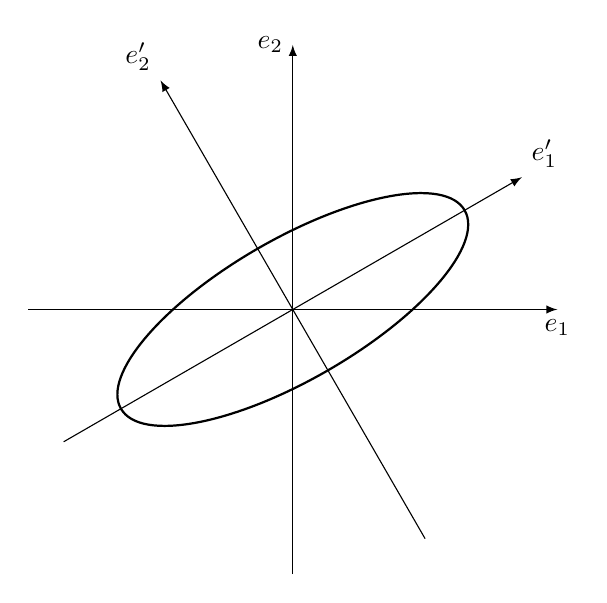
\begin{tikzpicture}[>=latex, scale=1.05]
  % 原坐标系 e_1, e_2
  \draw[->] (-3.2,0) -- (3.2,0) node[below]{$e_1$};
  \draw[->] (0,-3.2) -- (0,3.2) node[left]{$e_2$};
  
  \begin{scope}[rotate=30]
    % 椭圆
    \draw[thick] (0,0) ellipse (2.4 and 0.85);
    % 主轴新坐标系 e_1', e_2'
    \draw[->] (-3.2,0) -- (3.2,0) node[above right]{$e_1'$};
    \draw[->] (0,-3.2) -- (0,3.2) node[above left]{$e_2'$};
  \end{scope}
\end{tikzpicture}
\end{center}

\section{半双线性形式}\label{sec:7.1}

在下面的讨论中, 我们将只考虑系数域为 $\mathbb{R}$ 或 $\mathbb{C}$ 的向量空间, 并且通常用 $K$ 代替 $\mathbb{R}$ 或 $\mathbb{C}$ 来书写.特别是对 $\mathbb{C}$, 复\emph{共轭映射}(\textup{Konjugationsabbildung})\index{gongeyingshe@共轭映射(Konjugationsabbildung)}

\[
\mathbb{C} \longrightarrow \mathbb{C}, \qquad a \longmapsto \overline{a},
\]

将具有重要意义, 其中对 $a = \alpha + i \beta$($\alpha, \beta \in \mathbb{R}$), 相应的复共轭数由 $\overline{a} = \alpha - i \beta$ 给出.共轭映射 $a \longmapsto \overline{a}$ 表示 $\mathbb{C}$ 上的一个所谓的对合, 即一个满足 $\sigma^2 = \id$ 的自同构 $\sigma \colon \mathbb{C} \longrightarrow \mathbb{C}$, 并且还成立 $\sigma|_{\mathbb{R}} = \id$.对 $a = \alpha + i \beta \in \mathbb{C}$($\alpha, \beta \in \mathbb{R}$), 人们把

\[
\alpha = \frac{1}{2}(a + \overline{a}) = \operatorname{Re}(a)
\]

称为 $a$ 的实部, 把

\[
\beta = \frac{1}{2i}(a - \overline{a}) = \operatorname{Im}(a)
\]

称为 $a$ 的虚部, 并把

\[
|a| = \sqrt{\alpha^2 + \beta^2} = \sqrt{a \cdot \overline{a}}
\]

称为 $a$ 的绝对值.此时成立如下等价关系:

\[
a \in \mathbb{R} \Longleftrightarrow \operatorname{Re}(a) = a \Longleftrightarrow \operatorname{Im}(a) = 0 \Longleftrightarrow a = \overline{a}\text{.}
\]

对特殊元素 $a \in K$, 我们在后面也将考虑形如 $a \geq 0$ 或 $a > 0$ 的条件.这里的意思是 $a$ 为实数, 即满足 $a \in \mathbb{R} \subset K$, 并且此外满足条件 $a \geq 0$ 或 $a > 0$.

\begin{definition}[\emph{半双线性形式}\index{banshuangxianxingxingshi@半双线性形式(Sesquilinearform)}]\label{def:7.1.1}\index{banshuangxianxingxingshi@半双线性形式(Sesquilinearform)}
设 $V$ 是一个 $K$-向量空间.一个映射 $\varphi \colon V \times V \longrightarrow K$ 称为半双线性形式(sesqui = 一倍半), 如果对 $x, x_1, x_2, y, y_1, y_2 \in V$ 以及 $\alpha \in K$ 成立:
\begin{enumerate}
\item[(i)] $\varphi(x_1 + x_2, y) = \varphi(x_1, y) + \varphi(x_2, y)$;
\item[(ii)] $\varphi(\alpha x, y) = \alpha \varphi(x, y)$;
\item[(iii)] $\varphi(x, y_1 + y_2) = \varphi(x, y_1) + \varphi(x, y_2)$;
\item[(iv)] $\varphi(x, \alpha y) = \overline{\alpha} \varphi(x, y)$.
\end{enumerate}
\end{definition}

当 $K = \mathbb{R}$ 时恒有 $\alpha = \overline{\alpha}$, 此时人们也把它称为双线性形式 $\varphi$.如果满足

\[
\begin{array}{l}
\varphi(x, y) = 0 \ \text{对一切} \ y \in V \ \text{推出} \ x = 0, \\
\varphi(x, y) = 0 \ \text{对一切} \ x \in V \ \text{推出} \ y = 0,
\end{array}
\]

则称 $\varphi$ 为非退化的.

为得到一个简单的例子, 令 $V = K$.那么对固定的 $a \in K$, 由

\[
\varphi(x, y) = a \cdot x \cdot \overline{y}
\]

定义了 $V$ 上的一个半双线性形式, 并且它恰在 $a \neq 0$ 时非退化.

\begin{definition}[对称双线性形式与埃尔米特形式]\label{def:7.1.2}\index{shuangxianxingxingshi@双线性形式(Bilinearform)}\index{duichenshuangxianxingxingshi@对称双线性形式(symmetrische Bilinearform)}\index{aiermitexingshi@埃尔米特形式(hermitesche Form; HF)}
满足

\[
\varphi(x, y) = \overline{\varphi(y, x)} \quad \text{对一切} \quad x, y \in V
\]

的半双线性形式 $\varphi \colon V \times V \longrightarrow K$, 当 $K = \mathbb{R}$ 时称为对称双线性形式(简称 sBF), 当 $K = \mathbb{C}$ 时称为埃尔米特形式(简称 HF).对这样的形式, 人们经常用记号 $\langle x, y \rangle$ 代替 $\varphi(x, y)$.特别地, 此时对一切 $x \in V$ 成立 $\varphi(x, x) = \langle x, x \rangle \in \mathbb{R}$.
\end{definition}

例如,

\[
\varphi \colon K^n \times K^n \longrightarrow K, \qquad (x, y) \longmapsto x^t \cdot \overline{y},
\]

定义一个 sBF 或 HF, 其中这个映射详细写出来为:

\[
\bigl((x_1, \ldots, x_n)^t, (y_1, \ldots, y_n)^t\bigr) \longmapsto \sum_{i = 1}^{n} x_i \cdot \overline{y}_i\text{.}
\]

容易看出形式 $\varphi$ 是非退化的, 因为例如对 $x \neq 0$ 成立 $\varphi(x, x) > 0$.另一方面, 通过规定

\[
\bigl((x_1, \ldots, x_n)^t, (y_1, \ldots, y_n)^t\bigr) \longmapsto \sum_{i = 1}^{r} x_i \cdot \overline{y}_i,
\]

其中只求和到某个 $r < n$, 则在 $K^n$ 上定义了一个退化的形式.

\begin{definition}[\emph{正定}\index{zhengding@正定(positiv definit)}与数量积]\label{def:7.1.3}\index{zhengding@正定(positiv definit)}\index{shuliangji@数量积(Skalarprodukt)}
一个 sBF 或 HF $\varphi \colon V \times V \longrightarrow K$ 称为\emph{正半定}(\textup{positiv semi-definit})\index{zhengbanding@正半定(positiv semi-definit)}的, 如果对一切 $x \in V$ 成立 $\varphi(x, x) \geq 0$.如果甚至对一切 $x \in V - \{0\}$ 成立 $\varphi(x, x) > 0$, 则称 $\varphi$ 为正定的.此时人们也称 $\varphi$ 为 $V$ 上的一个数量积, 并把二元组 $(V, \varphi)$, 当 $K = \mathbb{R}$ 时称为\emph{欧几里得向量空间}(\textup{euklidischer Vektorraum})\index{oujilidexiangliangkongjian@欧几里得向量空间(euklidischer Vektorraum)}, 当 $K = \mathbb{C}$ 时称为酉向量空间.
\end{definition}

上面考察过的形式 $K^n \times K^n \longrightarrow K$, $(x, y) \longmapsto x^t \cdot \overline{y}$ 例如定义了 $K^n$ 上的一个数量积, 即所谓标准数量积.

\begin{theorem}[柯西-施瓦茨不等式]\label{thm:7.1.4}\index{kexishiwacibudengshi@柯西-施瓦茨不等式(Schwarz'sche Ungleichung)}
设 $\varphi \colon V \times V \longrightarrow K$, $(x, y) \longmapsto \langle x, y \rangle$ 是 $K$-向量空间 $V$ 上的正半定 sBF 或 HF.则对 $x, y \in V$ 成立下列不等式:

\[
|\langle x, y \rangle|^2 \leq \langle x, x \rangle \cdot \langle y, y \rangle\text{.}
\]

若 $\varphi$ 甚至正定, 则在这个公式中恰在 $x$ 与 $y$ 线性相关时成立等号.
\end{theorem}

\begin{proof}
任取 $\alpha, \beta \in K$.则成立

\[
\begin{array}{l}
0 \leq \langle \alpha x + \beta y, \alpha x + \beta y \rangle \\
= \alpha \overline{\alpha} \langle x, x \rangle + \alpha \overline{\beta} \langle x, y \rangle + \beta \overline{\alpha} \langle y, x \rangle + \beta \overline{\beta} \langle y, y \rangle \\
= \alpha \overline{\alpha} \langle x, x \rangle + 2\operatorname{Re}\bigl(\alpha \overline{\beta} \langle x, y \rangle\bigr) + \beta \overline{\beta} \langle y, y \rangle\text{.}
\end{array}
\]

若现在 $\langle x, x \rangle = \langle y, y \rangle = 0$, 则特别取 $\alpha = -1$ 与 $\beta = \langle x, y \rangle$.由此得

\[
0 \leq 2\operatorname{Re}\bigl(\alpha \overline{\beta} \langle x, y \rangle\bigr) = -2|\langle x, y \rangle|^2 \leq 0
\]

从而 $\langle x, y \rangle = 0$, 于是特别地

\[
|\langle x, y \rangle|^2 \leq \langle x, x \rangle \cdot \langle y, y \rangle\text{.}
\]

现在设 $\langle x, x \rangle > 0$.在此情形下取

\[
\alpha = -\overline{\langle x, y \rangle}, \qquad \beta = \langle x, x \rangle\text{.}
\]

于是得

\[
\begin{array}{c}
0 \leq |\langle x, y \rangle|^2 \langle x, x \rangle - 2|\langle x, y \rangle|^2 \langle x, x \rangle + \langle x, x \rangle^2 \langle y, y \rangle \\
= -|\langle x, y \rangle|^2 \langle x, x \rangle + \langle x, x \rangle^2 \langle y, y \rangle,
\end{array}
\]

即正如所期望的

\[
|\langle x, y \rangle|^2 \leq \langle x, x \rangle \cdot \langle y, y \rangle\text{.}
\]

情形 $\langle y, y \rangle > 0$ 可类似地处理.

若最后 $x, y \in V$ 线性相关, 则其中一个向量是另一个的倍数, 并且毫无困难地得到

\[
|\langle x, y \rangle|^2 = \langle x, x \rangle \cdot \langle y, y \rangle\text{.}
\]

反之, 若这个等式成立, 则如上取 $\alpha = -\overline{\langle x, y \rangle}$, $\beta = \langle x, x \rangle$ 得到

\[
\begin{array}{c}
\langle \alpha x + \beta y, \alpha x + \beta y \rangle \\
= |\langle x, y \rangle|^2 \langle x, x \rangle - 2|\langle x, y \rangle|^2 \langle x, x \rangle + \langle x, x \rangle^2 \langle y, y \rangle = 0\text{.}
\end{array}
\]

若 $\varphi$ 正定, 则由此得 $\alpha x + \beta y = 0$, 并且可以看到 $x, y$ 线性相关.因为对 $x = 0$ 这是显然的, 对 $x \neq 0$ 也如此, 因为此时系数 $\beta = \langle x, x \rangle$ 由 $\varphi$ 的正定性而不消失.
\end{proof}

\begin{corollary}\label{cor:7.1.5}
设 $\varphi \colon V \times V \longrightarrow K$ 是正半定 sBF 或 HF.则 $\varphi$ 正定, 当且仅当 $\varphi$ 非退化.
\end{corollary}

若 $\varphi \colon V \times V \longrightarrow K$ 是正半定 sBF 或 HF, 则对一切 $x \in V$ 成立 $\langle x, x \rangle \geq 0$, 并且人们把 $|x| = \sqrt{\langle x, x \rangle}$ 称为向量 $x \in V$(关于 $\varphi$)的长度或模长.如此定义的向量模长满足通常的三角不等式:

\begin{corollary}[三角不等式]\label{cor:7.1.6}\index{sanjiaobudengshi@三角不等式(Dreiecksungleichung)}
设 $\varphi \colon V \times V \longrightarrow K$ 是正半定 sBF 或 HF.则对 $x, y \in V$ 成立

\[
|x + y| \leq |x| + |y|\text{.}
\]
\end{corollary}

\begin{proof}
成立

\[
\begin{array}{r l}
|x + y|^2 & = \langle x + y, x + y \rangle \\
& = \langle x, x \rangle + 2\operatorname{Re}\bigl(\langle x, y \rangle\bigr) + \langle y, y \rangle \\
& \leq \langle x, x \rangle + 2|\langle x, y \rangle| + \langle y, y \rangle \\
& \leq |x|^2 + 2|x| \, |y| + |y|^2 \\
& = \bigl(|x| + |y|\bigr)^2
\end{array}
\]

从而 $|x + y| \leq |x| + |y|$.
\end{proof}

关于向量模长的进一步性质, 我们还可以列举: 对 $\alpha \in K$, $x \in V$ 成立 $|\alpha x| = |\alpha| \, |x|$.若 $\varphi$ 甚至正定, 则 $|x| = 0$ 等价于 $x = 0$.此外, 若 $\langle x, x \rangle = 1$ 从而 $|x| = 1$ 成立, 则称向量 $x \in V$ 为规范化的(normiert).例如对 $|x| \neq 0$ 的 $x \in V$, $\frac{x}{|x|}$ 是规范化的.

最后我们想借助几何直观解释 $\mathbb{R}^n$ 上的标准数量积.首先, 我们利用勾股定理确认, 向量 $x \in \mathbb{R}^n$ 的模长恰与点 $x$ 到原点的通常欧几里得距离一致.若 $e \in \mathbb{R}^n$ 是另一个向量且成立 $|e| = 1$, 则如下方程成立:

\[
|x|^2 = \langle x, e \rangle^2 + |x - \langle x, e \rangle e|^2\text{.}
\]

这容易直接验算.依据勾股定理的逆定理, 这在几何上意味着边长为 $|x|$, $|\langle x, e \rangle|$ 与 $|x - \langle x, e \rangle e|$ 的三角形是直角三角形:

\begin{center}
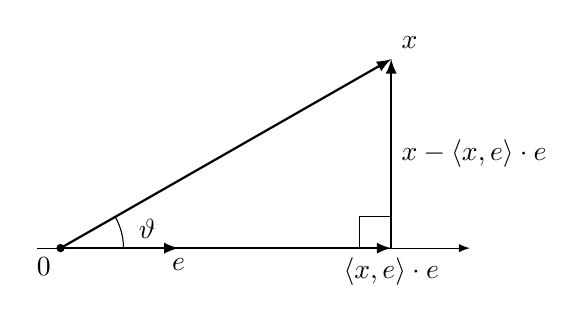
\begin{tikzpicture}[>=latex]
  \coordinate (O) at (0,0);
  \coordinate (E) at (1.5,0);
  \coordinate (P) at (4.2,0);
  \coordinate (X) at (4.2,2.4);
  
  \draw[->] (-0.3,0) -- (5.2,0);
  \draw[thick, ->] (O) -- (E) node[below]{$e$};
  \draw[thick, ->] (O) -- (P);
  \node[below] at (P) {$\langle x, e \rangle \cdot e$};
  
  \draw[thick, ->] (O) -- (X) node[above right]{$x$};
  \draw[thick, ->] (P) -- (X) node[midway, right]{$x - \langle x, e \rangle \cdot e$};
  
  % 直角标记
  \draw (3.8,0) -- (3.8,0.4) -- (4.2,0.4);
  
  % 夹角 vartheta
  \draw (0.8,0) arc (0:29.7:0.8);
  \node at (1.1,0.25) {$\vartheta$};
  
  \fill (O) circle (1.5pt) node[below left]{$0$};
\end{tikzpicture}
\end{center}

于是, 向量 $\langle x, e \rangle \cdot e$ 是这样产生的: 把 $x$ \emph{垂直投影}(\textup{senkrechte Projektion})\index{chuizhitouying@垂直投影(senkrechte Projektion)}到由 $e$ 给出的线性子空间 $\mathbb{R} \cdot e \subset \mathbb{R}^n$ 上.一般地, 可以按这种方式计算两个向量 $x, y \in \mathbb{R}^n - \{0\}$ 的数量积.即在上面的讨论中令 $e = |y|^{-1} \cdot y$.于是, 除符号外, $\langle x, y \rangle$ 作为 $|y|$ 与 $x$ 在直线 $\mathbb{R} \cdot y \subset \mathbb{R}^n$ 上的垂直投影的模长之积而得到.更准确地说, $x$ 在 $\mathbb{R} \cdot y$ 上的投影可以用分析学中的余弦函数来描述.若 $\vartheta$ 是 $x$ 与 $y$ 所夹的角, 则这个投影计算为 $\frac{|x|}{|y|} \cdot \cos(\vartheta) \cdot y$, 于是得:

\begin{theorem}\label{thm:7.1.7}
对向量 $x, y \in \mathbb{R}^n - \{0\}$ 与标准数量积成立

\[
\langle x, y \rangle = |x| \cdot |y| \cdot \cos \vartheta,
\]

其中 $\vartheta$ 是 $x$ 与 $y$ 所夹的角.
\end{theorem}

用 $x - \langle x, e \rangle e$ 从 $x$ 构造一个垂直于 $e$ 的向量, 这种可能性恰好就是我们在下面的 \ref{sec:7.2} 节中将要讨论的 E.~施密特正交规范化方法的中心思想.

\aufgaben

如无特别说明, 设 $V$ 是有限维 $\mathbb{R}$-向量空间, $\varphi \colon V \times V \longrightarrow \mathbb{R}$ 是 $V$ 上的对称双线性形式.

\medskip
\noindent\textbf{习题 1.} 通过

\[
\ker \varphi = \bigl\{x \in V;\, \varphi(x, y) = 0 \ \text{对一切} \ y \in V\bigr\}
\]

定义 $\varphi$ 的核, 并证明 $\varphi$ 在 $V/\ker \varphi$ 上诱导出一个非退化的对称双线性形式.

\medskip
\noindent\textbf{习题 2.} 通过令 $q(x) = \varphi(x, x)$($x \in V$)定义与 $\varphi$ 相应的二次型 $q \colon V \longrightarrow \mathbb{R}$, 并证明 $\varphi$ 由 $q$ 唯一确定.

\medskip
\noindent\textbf{习题 3.} 设 $\varphi$ 正定.对 $x, y \in V$, $y \neq 0$, 考虑 $t \in \mathbb{R}$ 的多项式函数 $p(t) = |x + ty|^2$.求出 $p(t)$ 的全部零点, 并由此推出当 $K = \mathbb{R}$ 时定理~\mtref{thm:7.1.4} 版本下的柯西-施瓦茨不等式.(AT 360)

\medskip
\noindent\textbf{习题 4.} 设 $\varphi$ 正定.对 $x, y \in V - \{0\}$ 证明:
\begin{enumerate}
\item[(i)] 成立 $-1 \leq \dfrac{\varphi(x, y)}{|x| \cdot |y|} \leq 1$.由分析学知存在一个角度 $0 \leq \vartheta \leq \pi$ 使得 $\dfrac{\varphi(x, y)}{|x| \cdot |y|} = \cos \vartheta$.
\item[(ii)] 成立余弦定理:
\end{enumerate}

\[
|x - y|^2 = |x|^2 + |y|^2 - 2|x| \, |y| \cos \vartheta\text{.}
\]

\medskip
\noindent\textbf{习题 5.} 设 $V$ 是系数域 $K$ 上的向量空间, $V^*$ 是其对偶空间, $W$ 是所有 $K$-双线性映射 $V \times V \longrightarrow K$ 构成的 $K$-向量空间.证明: 把同态 $\varphi \colon V \longrightarrow V^*$ 映为映射

\[
V \times V \longrightarrow K, \qquad (x, y) \longmapsto \varphi(x)(y)
\]

的映射 $\operatorname{Hom}_K(V, V^*) \longrightarrow W$ 是 $K$-向量空间的同构.(AT 361)

\section{正交性}\label{sec:7.2}

\begin{definition}[正交]\label{def:7.2.1}\index{zhengjiao@正交(orthogonal)}
设 $\varphi \colon V \times V \longrightarrow K$, $(x, y) \longmapsto \langle x, y \rangle$ 是一个 sBF 或 HF.若 $\langle x, y \rangle = 0$ 成立, 则称两个向量 $x, y \in V$ 互相正交或互相垂直.$V$ 中满足 $0 \notin M$ 的一个向量组 $M$ 称为\emph{正交系}(\textup{Orthogonalsystem})\index{zhengjiaoxi@正交系(Orthogonalsystem)}, 如果 $M$ 中任意两个向量都互相正交.若此外对一切 $x \in M$ 成立 $\langle x, x \rangle = 1$, 则也称其为\emph{标准正交系}(\textup{Orthonormalsystem})\index{biaozhunzhengjiaoxi@标准正交系(Orthonormalsystem)}.
\end{definition}

\begin{remark}\label{rem:7.2.2}
设 $\varphi \colon V \times V \longrightarrow K$ 是一个数量积.若 $M$ 是 $V$ 中向量的正交系, 则 $M$ 线性无关.
\end{remark}

\begin{proof}
对 $M$ 的一个有限子系统 $x_1, \ldots, x_n$ 考虑满足 $\sum_{i = 1}^{n} \alpha_i x_i = 0$ 的系数 $\alpha_1, \ldots, \alpha_n \in K$.于是对 $j = 1, \ldots, n$ 得

\[
0 = \Bigl\langle \sum_{i = 1}^{n} \alpha_i x_i, x_j \Bigr\rangle = \sum_{i = 1}^{n} \alpha_i \langle x_i, x_j \rangle = \alpha_j \langle x_j, x_j \rangle
\]

从而因 $\langle x_j, x_j \rangle > 0$ 得 $\alpha_j = 0$.
\end{proof}

\begin{definition}[正交基与标准正交基]\label{def:7.2.3}\index{zhengjiaoji@正交基(Orthogonalbasis)}\index{biaozhunzhengjiaoji@标准正交基(Orthonormalbasis)}
设 $\varphi \colon V \times V \longrightarrow K$ 是一个数量积.如果 $V$ 中向量 $e_1, \ldots, e_n$ 组成的组 $M$ 满足下列条件, 则称 $M$ 为 $V$ 的正交基(或标准正交基):
\begin{enumerate}
\item[(i)] $M$ 是 $V$ 的一个基;
\item[(ii)] $M$ 是一个正交系(或标准正交系).
\end{enumerate}
\end{definition}

把向量表示为某个标准正交基 $M = (e_1, \ldots, e_n)$ 中元素的线性组合后, 它们之间的数量积可以按简单的方式计算:

\[
\begin{array}{c}
\Bigl\langle \sum_{i = 1}^{n} \alpha_i e_i, \sum_{i = 1}^{n} \beta_i e_i \Bigr\rangle = \sum_{i, j = 1}^{n} \alpha_i \overline{\beta}_j \langle e_i, e_j \rangle \\
= \sum_{i, j = 1}^{n} \alpha_i \overline{\beta}_j \delta_{ij} = \sum_{i = 1}^{n} \alpha_i \overline{\beta}_i
\end{array}
\]

例如考虑 $K^n$ 上的标准数量积, 则 $K^n$ 的标准基构成一个标准正交基.

下面我们讨论所谓的 E.~施密特正交规范化方法, 借助它可以, 把欧几里得或酉向量空间中的基改造成标准正交基.首先我们处理这个方法的核心步骤, 即我们在 \ref{sec:7.1} 节末尾已经针对 $K^n$ 上的标准数量积做过几何说明的那个步骤.

\begin{lemma}[\emph{正交投影}\index{zhengjiaotouying@正交投影(orthogonale Projektion)}]\label{lem:7.2.4}\index{zhengjiaotouying@正交投影(orthogonale Projektion)}
设 $\varphi \colon V \times V \longrightarrow K$ 是一个数量积, $e_1, \ldots, e_k$ 是子空间 $U \subset V$ 的一个标准正交基.则

\[
p_U \colon V \longrightarrow U, \qquad x \longmapsto \sum_{j = 1}^{k} \langle x, e_j \rangle e_j,
\]

是一个满的 $K$-线性映射, 即所谓的到 $U$ 上的正交投影.它限制在 $U$ 上为恒等映射, 并且此外还满足方程 $\langle x - p_U(x), y \rangle = 0$($x \in V$, $y \in U$).由这个方程, $p_U$ 作为 $K$-线性映射 $V \longrightarrow U$ 被唯一确定.
\end{lemma}

\begin{proof}
由于形式 $\langle x, y \rangle$ 对 $x$ 是 $K$-线性的, 映射 $p_U$ 是 $K$-线性的.若又设 $x = \sum_{i = 1}^{k} \alpha_i e_i \in U$, 则

\[
\langle x, e_j \rangle = \Bigl\langle \sum_{i = 1}^{k} \alpha_i e_i, e_j \Bigr\rangle = \sum_{i = 1}^{k} \alpha_i \langle e_i, e_j \rangle = \alpha_j,
\]

并且特别地得 $p_U|_U = \id_U$.此外得

\[
\begin{array}{c}
\langle x - p_U(x), e_j \rangle = \langle x, e_j \rangle - \Bigl\langle \sum_{i = 1}^{k} \langle x, e_i \rangle e_i, e_j \Bigr\rangle \\
= \langle x, e_j \rangle - \langle x, e_j \rangle \langle e_j, e_j \rangle = 0,
\end{array}
\]

即 $x - p_U(x)$ 与 $e_1, \ldots, e_k$ 正交, 从而与 $U$ 正交.

若 $q_U \colon V \longrightarrow U$ 是任意一个满足 $\langle x - q_U(x), y \rangle = 0$($x \in V$, $y \in U$)的线性映射, 则特别地对 $x \in V$, $y \in U$ 成立 $\langle p_U(x) - q_U(x), y \rangle = 0$.由于 $V$ 的数量积限制为 $U$ 上的一个数量积, 必对 $x \in V$ 有 $p_U(x) - q_U(x) = 0$, 从而 $p_U = q_U$.
\end{proof}

若 $x_1, \ldots, x_n$ 是欧几里得或酉 $K$-向量空间的一个基, 那么可以先规范化 $x_1$, 即考虑向量 $e_1 = |x_1|^{-1} \cdot x_1$.然后可以依据引理~\mtref{lem:7.2.4} 作 $V$ 到子空间 $U_1 = K e_1$ 上的投影 $p_1$.向量 $e_2' = x_2 - p_1(x_2)$ 此时与 $e_1$ 正交, 并且 $e_1$ 连同 $|e_2'|^{-1} \cdot e_2'$ 组成一个标准正交系 $e_1, e_2$.按这种方式继续下去, 就可以把基 $x_1, \ldots, x_n$ 正交规范化, 即整体地转化为一个标准正交基.我们想把这一结果在这里更精确地表述并证明.

\begin{theorem}[施密特正交规范化]\label{thm:7.2.5}\index{zhengjiaoguifanhuafangfa@正交规范化方法(Schmidt'sches Orthonormalisierungsverfahren)}
设 $\varphi \colon V \times V \longrightarrow K$ 是一个数量积, $x_1, \ldots, x_n$ 是 $V$ 的一个基.则存在唯一确定的向量 $e_1, \ldots, e_n \in V$, 使得
\begin{enumerate}
\item[(i)] $e_1, \ldots, e_n$ 是 $V$ 的一个标准正交基;
\item[(ii)] 对 $k = 1, \ldots, n$ 成立 $\bigoplus_{i = 1}^{k} K e_i = \bigoplus_{i = 1}^{k} K x_i$;
\item[(iii)] 对 $E_k = (e_1, \ldots, e_k)$ 与 $X_k = (x_1, \ldots, x_k)$, 基变换矩阵 $A_k = A_{\id, E_k, X_k}$ 满足 $\det(A_k) > 0$, $k = 1, \ldots, n$.
\end{enumerate}

更准确地说, 诸向量 $e_k$($k = 1, \ldots, n$)可以按如下的归纳方式构造:

\[
e_k = \Bigl|x_k - \sum_{j = 1}^{k-1} \langle x_k, e_j \rangle e_j\Bigr|^{-1} \cdot \Bigl(x_k - \sum_{j = 1}^{k-1} \langle x_k, e_j \rangle e_j\Bigr)\text{.}
\]
\end{theorem}

\begin{proof}
我们首先证明存在性断言, 并对此对 $n$ 作归纳.归纳起点 $n = 0$ 是平凡的.设 $n > 0$, 并设 $e_1, \ldots, e_{n-1}$ 是具有所期望性质的 $U_{n-1} = \bigoplus_{i = 1}^{n-1} K x_i$ 的一个标准正交基.此时有 $x_n \notin U_{n-1} = \bigoplus_{i = 1}^{n-1} K e_i$, 故 $x_n - p_{n-1}(x_n)$ 不为零; 这里 $p_{n-1} \colon V \longrightarrow U_{n-1}$ 是依据引理~\mtref{lem:7.2.4} 的投影.于是

\[
e_n = \bigl|x_n - p_{n-1}(x_n)\bigr|^{-1} \cdot \bigl(x_n - p_{n-1}(x_n)\bigr)
\]

是良定义的, 并且由注记~\mtref{rem:7.2.2} 与引理~\mtref{lem:7.2.4} 可知 $e_1, \ldots, e_n$ 构成 $V$ 的一个标准正交基.此外, 由 $e_n$ 的定义存在形如

\[
e_n = \alpha \cdot x_n + y
\]

的方程, 其中常数 $\alpha > 0$, 向量 $y \in U_{n-1}$.由此得

\[
A_n = \begin{pmatrix} A_{n-1} & * \\ 0 & \alpha \end{pmatrix},
\]

并且由 $\alpha > 0$, $\det(A_{n-1}) > 0$ 得 $\det(A_n) = \alpha \cdot \det(A_{n-1}) > 0$.

为证明唯一性断言, 设 $f_1, \ldots, f_n$ 是 $V$ 的一个满足性质 (ii) 和 (iii) 的标准正交基.我们再次对 $n$ 作归纳来证明 $f_i = e_i$($i = 1, \ldots, n$), 其中归纳起点 $n = 0$ 是平凡的.设 $n > 0$.由归纳假设可以假定 $f_i = e_i$($i = 1, \ldots, n-1$).于是存在形如 $f_n = \alpha \cdot x_n + y$ 的方程, 其中 $\alpha \in K$, $y \in U_{n-1} = \bigoplus_{i = 1}^{n-1} K x_i$.基变换矩阵 $A_{\id, E', X}$, 其中我们使用基 $E' = (f_1, \ldots, f_n) = (e_1, \ldots, e_{n-1}, f_n)$ 与 $X = (x_1, \ldots, x_n)$, 此时具有形式

\[
A = \begin{pmatrix} A_{n-1} & * \\ 0 & \alpha \end{pmatrix},
\]

并且由 $\det(A)$, $\det(A_{n-1}) > 0$ 得 $\alpha > 0$.利用 $U_{n-1} = \bigoplus_{i = 1}^{n-1} K e_i$, 可以把 $y$ 写成 $e_1, \ldots, e_{n-1}$ 的线性组合.于是存在常数 $\beta_1, \ldots, \beta_{n-1} \in K$ 使得

\[
f_n = \alpha \cdot \Bigl(x_n - \sum_{i = 1}^{n-1} \beta_i e_i\Bigr)\text{.}
\]

对 $i = 1, \ldots, n-1$ 此时成立

\[
0 = \langle f_n, e_i \rangle = \alpha \cdot \bigl(\langle x_n, e_i \rangle - \beta_i\bigr),
\]

即 $\beta_i = \langle x_n, e_i \rangle$, 即

\[
f_n = \alpha \cdot \Bigl(x_n - \sum_{i = 1}^{n-1} \langle x_n, e_i \rangle e_i\Bigr)\text{.}
\]

由方程

\[
1 = |f_n| = \alpha \cdot \Bigl|x_n - \sum_{i = 1}^{n-1} \langle x_n, e_i \rangle e_i\Bigr|
\]

于是得

\[
\alpha = \Bigl|x_n - \sum_{i = 1}^{n-1} \langle x_n, e_i \rangle e_i\Bigr|^{-1}
\]

从而 $f_n = e_n$, 这正是所要证明的.
\end{proof}

\begin{corollary}\label{cor:7.2.6}
每个有限维欧几里得或酉向量空间 $V$ 都有一个标准正交基.子空间 $U \subset V$ 的每个标准正交基都可以扩充为 $V$ 的一个标准正交基.
\end{corollary}

\begin{corollary}\label{cor:7.2.7}
设 $V$ 是有限维欧几里得或酉向量空间, $V_1 \subset V_2 \subset \cdots \subset V_r = V$ 是 $K$-子空间的一个链.设 $\dim_K V_i = n_i$.则存在 $V$ 的一个标准正交基 $e_1, \ldots, e_n$, 使得 $e_1, \ldots, e_{n_i}$ 分别是 $V_i$ 的标准正交基, $i = 1, \ldots, r$.
\end{corollary}

若 $V$ 是带 sBF 或 HF 的 $K$-向量空间, 则当恒有 $\langle x, y \rangle = 0$($x \in M$, $y \in N$)时, 称两个子集 $M, N \subset V$ 正交, 记为 $M \perp N$.此时人们也写 $x \perp y$ 来代替 $\langle x, y \rangle = 0$, 其中 $x \perp y$ 等价于 $y \perp x$.此外, 对子集 $M \subset V$ 可以考察 $K$-子空间

\[
M^{\perp} = \bigl\{x \in V;\, x \perp y \ \text{对一切} \ y \in M\bigr\}\text{.}
\]

对子空间 $W \subset V$, 人们把 $W^{\perp}$ 称为 $W$ 在 $V$ 中的\emph{正交补}(\textup{orthogonales Komplement})\index{zhengjiaobu@正交补(orthogonales Komplement)}.

\begin{corollary}[正交补]\label{cor:7.2.8}\index{zhengjiaobu@正交补(orthogonales Komplement)}
设 $V$ 是有限维欧几里得或酉向量空间, $W \subset V$ 是一个子空间.则成立:
\begin{enumerate}
\item[(i)] $V = W \oplus W^{\perp}$, 特别地 $\dim_K W^{\perp} = \dim_K V - \dim_K W$;
\item[(ii)] $(W^{\perp})^{\perp} = W$.
\end{enumerate}
\end{corollary}

\begin{proof}
选取 $W$ 的一个标准正交基 $e_1, \ldots, e_r$, 并用元素 $e_{r+1}, \ldots, e_n$ 把它扩充为 $V$ 的一个标准正交基; 参见推论~\mtref{cor:7.2.6}.对 $W' = \bigoplus_{i = r+1}^{n} K e_i$ 此时成立 $W \perp W'$, 因而 $W' \subset W^{\perp}$.现在设 $x = \sum_{i = 1}^{n} \alpha_i e_i \in W^{\perp}$.方程 $\langle x, e_i \rangle = 0$($i = 1, \ldots, r$)此时表明 $\alpha_i = 0$($i = 1, \ldots, r$), 从而 $x \in W'$.因此成立 $W^{\perp} = W'$, 从而 $V = W \oplus W^{\perp}$.把这个论证应用于 $W^{\perp}$ 以代替 $W$, 便得到 $(W^{\perp})^{\perp} = W$.
\end{proof}

作为应用, 我们还想讨论 $\mathbb{R}^n$ 中平行多面体的体积.对线性无关的向量组 $x_1, \ldots, x_r \in \mathbb{R}^n$, 用

\[
P(x_1, \ldots, x_r) = \Bigl\{x \in \mathbb{R}^n;\, x = \sum_{i = 1}^{r} \alpha_i x_i \ \text{且} \ 0 \leq \alpha_i \leq 1\Bigr\}
\]

表示由这些向量张成的 $r$ 维平行多面体.若对 $r = n$, $x_1, \ldots, x_n$ 例如是 $\mathbb{R}^n$ 中的单位向量, 则 $P(x_1, \ldots, x_n)$ 恰为 $n$ 维单位立方体.

如通常一样, 我们把 $\mathbb{R}^n$ 看作带标准数量积的欧几里得向量空间.对一个 $r$ 维平行多面体 $P(x_1, \ldots, x_r)$, 考察由 $x_1, \ldots, x_r$ 生成的 $r$ 维子空间 $U \subset \mathbb{R}^n$, 并在 $U$ 中选取一个标准正交基 $M = (e_1, \ldots, e_r)$.然后设 $\det_M$ 是 $U$ 上在基 $M$ 上取值为 $1$ 的那个行列式函数; 参见定理~\mtref{thm:4.2.8}.在这种情形下, 平行多面体的体积定义为

\[
\operatorname{Vol}\bigl(P(x_1, \ldots, x_r)\bigr) = \bigl|\det_M(x_1, \ldots, x_r)\bigr|\text{.}
\]

自然要证明这个定义与 $U$ 的标准正交基 $M$ 的选取无关.我们还想说明, 这个体积与 $\mathbb{R}^n$ 中一个物体体积的直观观念一致.

\begin{theorem}[\emph{格拉姆行列式}\index{gelamuhanglieshi@格拉姆行列式(Gram'sche Determinante)}]\label{thm:7.2.9}\index{gelamuhanglieshi@格拉姆行列式(Gram'sche Determinante)}
对向量 $x_1, \ldots, x_r \in K^n$, 相应的格拉姆行列式定义为

\[
G(x_1, \ldots, x_r) = \det \begin{pmatrix}
\langle x_1, x_1 \rangle & \cdots & \langle x_1, x_r \rangle \\
\vdots & & \vdots \\
\langle x_r, x_1 \rangle & \cdots & \langle x_r, x_r \rangle
\end{pmatrix}
\]

其中 $\langle \cdot, \cdot \rangle$ 是 $K^n$ 上的标准数量积.成立 $G(x_1, \ldots, x_r) \geq 0$, 且 $G(x_1, \ldots, x_r)$ 恰在 $x_1, \ldots, x_r$ 线性相关时消失.

若 $x_1, \ldots, x_r$ 线性无关, $M = (e_1, \ldots, e_r)$ 是 $x_1, \ldots, x_r$ 在 $K^n$ 中生成的线性子空间的一个标准正交基, 则成立关系式

\[
G(x_1, \ldots, x_r) = \bigl|\det_M(x_1, \ldots, x_r)\bigr|^2\text{.}
\]
\end{theorem}

注意, 这个断言在 $r = 2$ 时恰好给出柯西-施瓦茨不等式(定理~\mtref{thm:7.1.4}), 而且独立于定理~\mtref{thm:7.1.4} 中给出的证明.此外我们还可以断言:

\begin{corollary}[平行多面体的体积]\label{cor:7.2.10}
平行多面体 $P(x_1, \ldots, x_r) \subset \mathbb{R}^n$ 的体积是良定义的, 且成立

\[
\operatorname{Vol}\bigl(P(x_1, \ldots, x_r)\bigr) = G(x_1, \ldots, x_r)^{\frac{1}{2}}\text{.}
\]
\end{corollary}

\begin{proof}[定理~\mtref{thm:7.2.9} 的证明]
若 $x_1, \ldots, x_r$ 线性相关, 则立即看出格拉姆行列式矩阵中的列或行线性相关, 故成立 $G(x_1, \ldots, x_r) = 0$.因此设 $x_1, \ldots, x_r$ 线性无关.于是这些向量生成一个 $r$ 维子空间 $U \subset K^n$, 它同样配备有数量积, 并且我们可以依据定理~\mtref{thm:7.2.5} 在 $U$ 中选取一个标准正交基 $M = (e_1, \ldots, e_r)$.若再用 $x_{1, M}, \ldots, x_{r, M}$ 表示 $x_1, \ldots, x_r$ 关于基 $M$ 的坐标列向量, 则成立

\[
(x_{1, M}, \ldots, x_{r, M})^t \cdot (\overline{x}_{1, M}, \ldots, \overline{x}_{r, M}) = \bigl(\langle x_i, x_j \rangle\bigr)_{i, j = 1, \ldots, r}\text{.}
\]

特别地得

\[
\bigl|\det_M(x_1, \ldots, x_r)\bigr|^2 = \bigl|\det(x_{1, M}, \ldots, x_{r, M})\bigr|^2 = G(x_1, \ldots, x_r)
\]

从而由 $x_1, \ldots, x_r$ 线性无关得 $G(x_1, \ldots, x_r) > 0$.
\end{proof}

现在我们还想说明, 平行多面体的上述体积

\[
\operatorname{Vol}\bigl(P(x_1, \ldots, x_r)\bigr) = \bigl|\det_M(x_1, \ldots, x_r)\bigr| = G(x_1, \ldots, x_r)^{\frac{1}{2}}
\]

(其中 $M = (e_1, \ldots, e_r)$ 是 $x_1, \ldots, x_r$ 在 $\mathbb{R}^n$ 中生成的子空间的一个标准正交基)在直观意义下也恰好对应 $P(x_1, \ldots, x_r)$ 的 $r$ 维体积.对 $r = 1$ 这是立即明白的.对 $r > 1$ 考察正交投影 $p_U \colon \mathbb{R}^n \longrightarrow U := \sum_{i = 1}^{r-1} \mathbb{R} x_i$.此时 $x_r' = x_r - p_U(x_r)$ 与 $U$ 正交, 从而与 $x_1, \ldots, x_{r-1}$ 正交.于是成立

\[
\begin{array}{c}
\operatorname{Vol}\bigl(P(x_1, \ldots, x_r)\bigr) = \bigl|\det_M(x_1, \ldots, x_r)\bigr| \\
= \bigl|\det_M(x_1, \ldots, x_{r-1}, x_r')\bigr| = \operatorname{Vol}\bigl(P(x_1, \ldots, x_{r-1}, x_r')\bigr)
\end{array}
\]

以及

\[
\begin{array}{l}
\operatorname{Vol}\bigl(P(x_1, \ldots, x_r)\bigr)^2 = \operatorname{Vol}\bigl(P(x_1, \ldots, x_{r-1}, x_r')\bigr)^2 \\
\qquad = \det \begin{pmatrix}
\langle x_1, x_1 \rangle & \cdots & \langle x_1, x_{r-1} \rangle & 0 \\
\vdots & \ddots & \vdots & \vdots \\
\langle x_{r-1}, x_1 \rangle & \cdots & \langle x_{r-1}, x_{r-1} \rangle & 0 \\
0 & \cdots & 0 & \langle x_r', x_r' \rangle
\end{pmatrix} \\
\qquad = \det \begin{pmatrix}
\langle x_1, x_1 \rangle & \cdots & \langle x_1, x_{r-1} \rangle \\
\vdots & \ddots & \vdots \\
\langle x_{r-1}, x_1 \rangle & \cdots & \langle x_{r-1}, x_{r-1} \rangle
\end{pmatrix} \cdot |x_r'|^2 \\
\qquad = \operatorname{Vol}\bigl(P(x_1, \ldots, x_{r-1})\bigr)^2 \cdot |x_r'|^2\text{.}
\end{array}
\]

现在 $|x_r'|$ 应解释为 $x_r$ 到 $U$ 的垂直距离; 关于这一点也参见本节末尾的习题 4.于是 $r$ 维平行多面体 $P(x_1, \ldots, x_r)$ 的体积, 作为 $(r-1)$ 维"底面"$P(x_1, \ldots, x_{r-1})$ 的体积与 $x_r$ 在此底面上方的"高"之积而得到.由归纳立刻可知, 平行多面体的上述体积与具有相同高度比的立方体的体积一致, 这与直观观念相符.

\aufgaben

\medskip
\noindent\textbf{习题 1.} 把 $\mathbb{R}^3$ 看作带标准数量积的欧几里得向量空间, 并把 E.~施密特正交规范化方法应用于基 $(1, 1, 0)$, $(1, 0, 1)$, $(0, 1, 1) \in \mathbb{R}^3$.

\medskip
\noindent\textbf{习题 2.} 对 $n \in \mathbb{N}$ 设 $\mathbb{R}[T]_n \subset \mathbb{R}[T]$ 是所有次数 $\leq n$ 的多项式构成的 $\mathbb{R}$-子空间.证明: 通过

\[
\langle f, g \rangle = \int_{0}^{1} f(t) g(t) \, dt, \qquad f, g \in \mathbb{R}[T]_n,
\]

在 $\mathbb{R}[T]_n$ 上定义了一个数量积.对 $n = 2$, 把 E.~施密特正交规范化方法应用于 $\mathbb{R}[T]_2$ 的基 $1, T, T^2$.(AT 362)

\medskip
\noindent\textbf{习题 3.} 设 $V$ 是带基 $x_1, \ldots, x_n$ 的欧几里得或酉 $K$-向量空间, 通过对它应用 E.~施密特正交规范化方法得到标准正交基 $e_1, \ldots, e_n$.对满足 $|\varepsilon_i| = 1$ 的常数 $\varepsilon_1, \ldots, \varepsilon_n \in K$, 证明: 正交规范化方法把基 $\varepsilon_1 x_1, \ldots, \varepsilon_n x_n$ 转化为标准正交基 $\varepsilon_1 e_1, \ldots, \varepsilon_n e_n$.

\medskip
\noindent\textbf{习题 4.} 设 $V$ 是欧几里得或酉 $K$-向量空间, $U \subset V$ 是一个子空间, $v \in V - U$.证明 (AT 363):
\begin{enumerate}
\item[(i)] 存在唯一一个 $u_0 \in U$ 使得 $v - u_0 \in U^{\perp}$;
\item[(ii)] 对一切满足 $u \neq u_0$ 的 $u \in U$ 成立 $|v - u| > |v - u_0|$.
\end{enumerate}

\medskip
\noindent\textbf{习题 5.} 设 $V = \mathbb{R}^{n \times n}$ 是所有实 $(n \times n)$-矩阵构成的 $\mathbb{R}$-向量空间.证明:
\begin{enumerate}
\item[(i)] 通过 $\varPhi(A, B) = \operatorname{Spur}(A \cdot B)$(即矩阵 $A \cdot B$ 的迹)在 $V$ 上定义了一个非退化的对称双线性形式.
\item[(ii)] 设 $U_{+} = \{U \in V;\, U^t = U\}$ 是所有对称矩阵构成的子空间, $U_{-} = \{U \in V;\, U^t = -U\}$ 是所有斜对称矩阵构成的子空间.成立
\end{enumerate}

\[
V = U_{+} \oplus U_{-}, \qquad U_{+}^{\perp} = U_{-}, \qquad U_{-}^{\perp} = U_{+}\text{.}
\]

\begin{enumerate}
\item[(iii)] $\varPhi$ 在 $U_{+}$ 上正定, 在 $U_{-}$ 上负定, 即对一切 $A \in U_{+} - \{0\}$ 成立 $\varPhi(A, A) > 0$, 对一切 $A \in U_{-} - \{0\}$ 成立 $\varPhi(A, A) < 0$.
\end{enumerate}

\section{半双线性形式与矩阵}\label{sec:7.3}

对矩阵 $A = (\alpha_{ij})_{i = 1, \ldots, m} \in K^{m \times n}$, 人们把

\[
\overline{A} = (\overline{\alpha}_{ij})_{\substack{i = 1, \ldots, m\\ j = 1, \ldots, n}} \in K^{m \times n}
\]

称为 $A$ 的共轭矩阵, 把

\[
A^{t} = (\alpha_{ij})_{\substack{j = 1, \ldots, n\\ i = 1, \ldots, m}} \in K^{n \times m}
\]

称为 $A$ 的转置矩阵, 并把

\[
A^{*} = \overline{A}^{t} = (\overline{\alpha}_{ij})_{\substack{j = 1, \ldots, n\\ i = 1, \ldots, m}} \in K^{n \times m}
\]

称为 $A$ 的伴随矩阵.这里要注意, "伴随"这一称谓的含义与 \ref{sec:4.4} 节中的不同.关于共轭矩阵的运算, 成立下列法则; 设 $A$, $B$ 是矩阵, $c \in K$ 是一个常数:

\[
\begin{array}{c}
\overline{A + B} = \overline{A} + \overline{B} \\
\overline{c \cdot A} = \overline{c} \cdot \overline{A} \\
\overline{A \cdot B} = \overline{A} \cdot \overline{B} \\
\overline{A^{-1}} = (\overline{A})^{-1} \\
\det(\overline{A}) = \overline{\det(A)}
\end{array}
\]

关于矩阵的转置, 我们已经知道下列运算法则:

\[
\begin{array}{c}
(A + B)^{t} = A^{t} + B^{t} \\
(c \cdot A)^{t} = c \cdot A^{t} \\
(A \cdot B)^{t} = B^{t} \cdot A^{t} \\
(A^{-1})^{t} = (A^{t})^{-1} \\
\det(A^{t}) = \det(A)
\end{array}
\]

其中前两个等式由注记~\mtref{rem:3.2.6} 得出, 第三个,以及作为简单推论的第四个由注记~\mtref{rem:3.2.8} 得出, 最后一个是定理~\mtref{thm:4.3.4}.于是关于伴随矩阵的运算得到下列法则:

\[
\begin{array}{c}
(A + B)^{*} = A^{*} + B^{*} \\
(c \cdot A)^{*} = \overline{c} \cdot A^{*} \\
(A \cdot B)^{*} = B^{*} \cdot A^{*} \\
(A^{-1})^{*} = (A^{*})^{-1} \\
\det(A^{*}) = \overline{\det(A)}
\end{array}
\]

下面我们想借助矩阵来描述半双线性形式.

\begin{definition}[半双线性形式的矩阵]\label{def:7.3.1}
设 $\varphi \colon V \times V \longrightarrow K$ 是带基 $X = (x_1, \ldots, x_n)$ 的 $K$-向量空间 $V$ 上的半双线性形式.则

\[
A_{\varphi, X} = \bigl(\varphi(x_i, x_j)\bigr)_{i, j = 1, \ldots, n} \in K^{n \times n}
\]

称为属于 $\varphi$,关于基 $X$ 的矩阵.
\end{definition}

\begin{theorem}\label{thm:7.3.2}
设 $\varphi \colon V \times V \longrightarrow K$ 是带基 $X = (x_1, \ldots, x_n)$ 的 $K$-向量空间 $V$ 上的半双线性形式.若如通常那样用 $a_X$ 表示向量 $a \in V$ 的坐标列向量, 则对 $a, b \in V$ 成立

\[
\varphi(a, b) = a_X^{t} \cdot A_{\varphi, X} \cdot \overline{b}_X,
\]

并且矩阵 $A_{\varphi, X} \in K^{n \times n}$ 由这个关系唯一刻画.此外, $\varphi$ 非退化, 当且仅当 $\det(A_{\varphi, X}) \neq 0$ 成立.
\end{theorem}

\begin{proof}
设 $a = \sum_{i = 1}^{n} \alpha_i x_i$, $b = \sum_{j = 1}^{n} \beta_j x_j$.于是得

\[
\varphi(a, b) = \sum_{i, j = 1}^{n} \alpha_i \cdot \varphi(x_i, x_j) \cdot \overline{\beta}_j = a_X^{t} \cdot A_{\varphi, X} \cdot \overline{b}_X,
\]

正如所断言的.另一方面, 若有一个矩阵 $A = (\alpha_{ij})_{i, j} \in K^{n \times n}$ 使得对 $a, b \in V$ 成立

\[
\varphi(a, b) = a_X^{t} \cdot A \cdot \overline{b}_X,
\]

则把 $x_1, \ldots, x_n$ 分别代入 $a$ 或 $b$, 得

\[
\varphi(x_i, x_j) = \alpha_{ij}
\]

从而 $A = A_{\varphi, X}$, 即矩阵 $A = A_{\varphi, X}$ 由上述关系唯一确定.

现在设 $\varphi$ 退化, 比如说在第一个变元上退化.即设 $a \in V$ 不为零且对一切 $b \in V$ 成立 $\varphi(a, b) = 0$.则

\[
a_X^{t} \cdot A_{\varphi, X} \cdot \overline{b}_X = 0 \quad \text{对一切} \quad b \in V\text{.}
\]

把这应用于 $b = x_1, \ldots, x_n$, 得到 $a_X^{t} \cdot A_{\varphi, X} = 0$.$K$-线性映射

\[
K^n \longrightarrow K^n, \qquad x \longmapsto A_{\varphi, X}^{t} \cdot x,
\]

因此具有非平凡的核, 并由定理~\mtref{thm:4.3.4} 得

\[
\det(A_{\varphi, X}) = \det(A_{\varphi, X}^{t}) = 0\text{.}
\]

反之, 借助推论~\mtref{cor:2.1.11} 与定理~\mtref{thm:4.3.4}, 从这样的等式推出 $\varphi$ 在第一个变元上退化.$\varphi$ 在第二个变元上退化的情形可以类似地处理.
\end{proof}

上面的证明还更精确地表明了:

\begin{corollary}\label{cor:7.3.3}
设 $V$ 是带基 $X$ 的有限维 $K$-向量空间.则对应 $\varphi \longmapsto A_{\varphi, X}$ 定义了所有半双线性形式 $\varphi \colon V \times V \longrightarrow K$ 的集合与所有 $(n \times n)$-矩阵 $K^{n \times n}$ 的集合之间的双射.此外, 对这样的半双线性形式 $\varphi$, 下列条件等价:
\begin{enumerate}
\item[(i)] $\varphi(a, b) = 0$ 对一切 $b \in V$ 推出 $a = 0$;
\item[(ii)] $\varphi(a, b) = 0$ 对一切 $a \in V$ 推出 $b = 0$;
\item[(iii)] $\varphi$ 非退化;
\item[(iv)] $\det(A_{\varphi, X}) \neq 0$.
\end{enumerate}
\end{corollary}

\begin{corollary}\label{cor:7.3.4}
设 $\varphi \colon V \times V \longrightarrow K$ 是带基 $X$ 的有限维 $K$-向量空间 $V$ 上的半双线性形式.则下列条件等价:
\begin{enumerate}
\item[(i)] $\varphi$ 是一个 sBF 或 HF, 即对一切 $a, b \in V$ 成立 $\varphi(a, b) = \overline{\varphi(b, a)}$;
\item[(ii)] $A_{\varphi, X} = (A_{\varphi, X})^{*}$.
\end{enumerate}
\end{corollary}

\begin{proof}
对 $a, b \in V$ 成立

\[
\begin{array}{c}
\overline{\varphi(b, a)} = \overline{\bigl(b_X^{t} \cdot A_{\varphi, X} \cdot \overline{a}_X\bigr)} = \overline{b}_X^{t} \cdot \overline{A}_{\varphi, X} \cdot a_X \\
= \bigl(\overline{b}_X^{t} \cdot \overline{A}_{\varphi, X} \cdot a_X\bigr)^{t} = a_X^{t} \cdot (A_{\varphi, X})^{*} \cdot \overline{b}_X\text{.}
\end{array}
\]

由定理~\mtref{thm:7.3.2}, 方程 $\varphi(a, b) = \overline{\varphi(b, a)}$($a, b \in V$)因此等价于 $A_{\varphi, X} = (A_{\varphi, X})^{*}$.
\end{proof}

下面我们想研究, $V$ 中的基变换如何影响半双线性形式 $\varphi \colon V \times V \longrightarrow K$ 的描述矩阵 $A_{\varphi, X}$.在 \ref{sec:3.4} 节中我们曾对 $V$ 的给定基 $Y$ 和 $X$ 考察过形如 $A_{\id, Y, X}$ 的基变换矩阵.我们在下面将缩写地写 $A_{Y, X}$ 来代替 $A_{\id, Y, X}$.

\begin{theorem}\label{thm:7.3.5}
设 $\varphi \colon V \times V \longrightarrow K$ 是带基 $X$ 和 $Y$ 的有限维 $K$-向量空间 $V$ 上的半双线性形式.则成立

\[
A_{\varphi, Y} = A_{Y, X}^{t} \cdot A_{\varphi, X} \cdot \overline{A}_{Y, X}\text{.}
\]
\end{theorem}

\begin{proof}
对 $a \in V$ 有 $a_X = A_{Y, X} \cdot a_Y$, 从而对 $a, b \in V$ 有

\[
\begin{array}{r l}
\varphi(a, b) & = a_X^{t} \cdot A_{\varphi, X} \cdot \overline{b}_X \\
& = (A_{Y, X} \cdot a_Y)^{t} \cdot A_{\varphi, X} \cdot \overline{A_{Y, X} \cdot b_Y} \\
& = a_Y^{t} \cdot A_{Y, X}^{t} \cdot A_{\varphi, X} \cdot \overline{A}_{Y, X} \cdot \overline{b}_Y
\end{array}
\]

因而依据定理~\mtref{thm:7.3.2} 得 $A_{\varphi, Y} = A_{Y, X}^{t} \cdot A_{\varphi, X} \cdot \overline{A}_{Y, X}$.
\end{proof}

\begin{corollary}\label{cor:7.3.6}
设 $\varphi \colon V \times V \longrightarrow K$ 是带基 $X = (x_1, \ldots, x_n)$ 的 $K$-向量空间 $V$ 上的半双线性形式.则下列条件等价:
\begin{enumerate}
\item[(i)] $\varphi$ 是一个数量积, 即一个正定 sBF 或 HF;
\item[(ii)] 存在矩阵 $S \in \mathrm{Gl}(n, K)$, 使得成立:
\end{enumerate}

\[
S^{t} \cdot A_{\varphi, X} \cdot \overline{S} = E
\]

其中 $E \in K^{n \times n}$ 是单位矩阵.
\end{corollary}

\begin{proof}
首先设 $\varphi$ 是一个数量积.则由定理~\mtref{thm:7.2.5}, $V$ 有一个标准正交基 $Y$.于是成立 $A_{\varphi, Y} = E$, 并由定理~\mtref{thm:7.3.5} 以 $S = A_{Y, X}$ 得到 $S^{t} \cdot A_{\varphi, X} \cdot \overline{S} = E$.

反之, 若对某个 $S \in \mathrm{Gl}(n, K)$ 成立 $S^{t} \cdot A_{\varphi, X} \cdot \overline{S} = E$, 则可以把 $S$ 看作 $A_{Y, X}$ 型的基变换矩阵, 从而成立 $A_{\varphi, Y} = E$.此时 $\varphi$ 是一个数量积.
\end{proof}

上述推论特别地包含这样的断言: 正定 sBF 或 HF 的描述矩阵 $A_{\varphi, X}$ 可以通过变换基 $X$ 化为单位矩阵, 即通过过渡到标准正交基.若去掉正定这一前提, 那么正如我们将在 7.6/6 中证明的, 仍然可以化 $A_{\varphi, X}$ 为实对角矩阵.

\begin{corollary}\label{cor:7.3.7}
若 $\varphi \colon V \times V \longrightarrow K$ 是有限维 $K$-向量空间 $V$ 上的数量积, 则对 $V$ 的一切基 $X$ 成立 $\det(A_{\varphi, X}) > 0$.
\end{corollary}

\begin{proof}
设 $X$ 是 $V$ 的一个标准正交基; 参见定理~\mtref{thm:7.2.5}; 此时成立 $A_{\varphi, X} = E$.对 $V$ 的另一个基 $Y$, 利用定理~\mtref{thm:7.3.5} 中的等式得到

\[
\begin{array}{c}
\det(A_{\varphi, Y}) = \det(A_{Y, X}^{t}) \cdot \det(A_{\varphi, X}) \cdot \det(\overline{A_{Y, X}}) \\
= \det(A_{Y, X}) \cdot \overline{\det(A_{Y, X})} = \bigl|\det(A_{Y, X})\bigr|^2 > 0,
\end{array}
\]

因为 $\det(A_{Y, X}) \neq 0$.
\end{proof}

最后我们还想给出 sBF 或 HF 正定性的一个行列式判别准则.

\begin{theorem}[\emph{主子式}\index{zhuzishi@主子式(Hauptunterdeterminanten)}判别准则]\label{thm:7.3.8}\index{zhuzishi@主子式(Hauptunterdeterminanten)}
设 $\varphi \colon V \times V \longrightarrow K$ 是带基 $X = (x_1, \ldots, x_n)$ 的 $K$-向量空间 $V$ 上的 sBF 或 HF.考察矩阵

\[
A_{r} = \bigl(\varphi(x_i, x_j)\bigr)_{i, j = 1, \ldots, r} \in K^{r \times r}, \qquad r = 1, \ldots, n\text{.}
\]

则下列条件等价:
\begin{enumerate}
\item[(i)] $\varphi$ 正定, 从而是一个数量积;
\item[(ii)] 对 $r = 1, \ldots, n$ 成立 $\det(A_r) > 0$.
\end{enumerate}
\end{theorem}

\begin{proof}
蕴含关系 (i) $\Longrightarrow$ (ii) 容易看出.把 $\varphi$ 限制到子空间 $V_r = \sum_{i = 1}^{r} K x_i$($r = 1, \ldots, n$)上.推论~\mtref{cor:7.3.7} 此时表明 $\det(A_r) > 0$.

为证明逆方向, 我们假定对 $r = 1, \ldots, n$ 成立 $\det(A_r) > 0$, 并通过对 $n$ 作归纳证明 $\varphi$ 是一个数量积.情形 $n = 1$ 是平凡的, 因为此时 $x_1$ 是 $V$ 的一个基, 并且成立 $\varphi(x_1, x_1) = \det(A_1) > 0$.设 $n > 1$.则由归纳假设 $\varphi|_{V_{n-1}}$ 正定, 并且由定理~\mtref{thm:7.2.5}, $V_{n-1}$ 有一个标准正交基 $e_1, \ldots, e_{n-1}$.此外, 如引理~\mtref{lem:7.2.4} 的证明那样容易看出, $e_1, \ldots, e_{n-1}$ 连同

\[
x_n' = x_n - \sum_{i = 1}^{n-1} \varphi(x_n, e_i) e_i
\]

组成 $V$ 的一个正交基 $Y$, 其中成立

\[
A_{\varphi, Y} = \begin{pmatrix}
1 & & & 0 \\
& \ddots & & \\
& & 1 & 0 \\
0 & & 0 & \varphi(x_n', x_n')
\end{pmatrix}
\]

以 $S = A_{Y, X}$ 则由定理~\mtref{thm:7.3.5} 得 $A_{\varphi, Y} = S^{t} A_n \overline{S}$, 从而

\[
\varphi(x_n', x_n') = \det(A_{\varphi, Y}) = |\det(S)|^2 \cdot \det(A_n) > 0\text{.}
\]

因此若令

\[
e_n = \frac{1}{\sqrt{\varphi(x_n', x_n')}} \cdot x_n',
\]

则成立 $\varphi(e_n, e_n) = 1$, 并且 $e_1, \ldots, e_n$ 组成 $V$ 的一个标准正交基.特别地 $\varphi$ 正定.
\end{proof}

在定理~\mtref{thm:7.3.8} 的情形中, 人们也把行列式 $\det(A_r)$($r = 1, \ldots, n$)称为矩阵 $A_{\varphi, X}$ 的主子式.把推论~\mtref{cor:7.3.4} 与定理~\mtref{thm:7.3.8} 结合起来, 便得到:

\begin{corollary}\label{cor:7.3.9}
对矩阵 $A \in K^{n \times n}$ 考察半双线性形式

\[
\varphi \colon K^n \times K^n \longrightarrow K, \qquad (a, b) \longmapsto a^{t} \cdot A \cdot \overline{b}\text{.}
\]

则下列条件等价:
\begin{enumerate}
\item[(i)] $\varphi$ 是一个数量积;
\item[(ii)] $A = A^{*}$ 且 $A$ 的所有主子式均为正.
\end{enumerate}
\end{corollary}

\aufgaben

$V$ 恒为维数 $n < \infty$ 的 $K$-向量空间.

\medskip
\noindent\textbf{习题 1.} 证明: 在 $V \times V$ 上 $K$-值函数的加法与纯量乘法之下, 所有半双线性形式 $V \times V \longrightarrow K$ 的集合构成一个 $K$-向量空间, 特别地也构成一个 $\mathbb{R}$-向量空间.分别计算维数.下列子集中哪些构成 $\mathbb{R}$ 或 $\mathbb{C}$ 上的线性子空间? 在可能的情形下计算相应的维数.
\begin{enumerate}
\item[(i)] 当 $K = \mathbb{R}$ 时的对称双线性形式;
\item[(ii)] 当 $K = \mathbb{C}$ 时的埃尔米特形式;
\item[(iii)] 数量积.
\end{enumerate}

\medskip
\noindent\textbf{习题 2.} 在 $\dim V \geq 2$ 的情形, 在 $V$ 上构造一个非退化的 sBF 或 HF $\varphi$ 以及一个非平凡线性子空间 $U \subset V$, 使得 $\varphi|_{U \times U}$ 退化.

\medskip
\noindent\textbf{习题 3.} 设 $\varphi$ 是 $V$ 上正半定的 sBF 或 HF.证明: 存在 $V$ 的一个基 $X$, 使得相应的矩阵 $A_{\varphi, X}$ 是主对角线元素为 $1$ 或 $0$ 的对角矩阵, 即 $A_{\varphi, X} = \operatorname{Diag}(1, \ldots, 1, 0, \ldots, 0)$.

\medskip
\noindent\textbf{习题 4.} 设 $\varphi$ 是 $V$ 上的 sBF 或 HF, $X$ 是 $V$ 的一个基.证明: 若 $\varphi$ 正半定, 则 $A_{\varphi, X}$ 的所有主子式都是实数 $\geq 0$.逆命题也成立吗? (AT 364)

\medskip
\noindent\textbf{习题 5.} 对矩阵 $A \in K^{n \times n}$, 恰好当 $A$ 的列(或行)在 $K^n$ 中组成一个标准正交基时成立 $A^{*} = A^{-1}$.这样的矩阵称为正交的(当 $K = \mathbb{R}$)或酉的(当 $K = \mathbb{C}$).

\medskip
\noindent\textbf{习题 6.} 设 $\varphi$ 是 $V$ 上的一个数量积.对 $V$ 上每一个另外的数量积 $\psi$, 证明: 存在自同态 $f \colon V \longrightarrow V$, 使得对一切 $x, y \in V$ 成立 $\psi(x, y) = \varphi(f(x), f(y))$.

\medskip
\noindent\textbf{习题 7.} 对矩阵 $A \in K^{n \times n}$ 证明: 通过 $\langle a, b \rangle = a^{t} \cdot A \cdot \overline{b}$ 在 $K^n$ 上定义了一个数量积, 当且仅当存在矩阵 $S \in \mathrm{Gl}(n, K)$ 使得 $A = S^{t} \cdot \overline{S}$.(AT 365)

% 第 7 章 7.4--7.6 节: 伴随映射, 等距同构与正交/酉矩阵, 自伴随映射
% 原书: Siegfried Bosch, Lineare Algebra, 7.4 Die adjungierte Abbildung,
%       7.5 Isometrien, orthogonale und unitäre Matrizen,
%       7.6 Selbstadjungierte Abbildungen

\section{伴随映射}\index{bansuiyingshe@伴随映射(adjungierte Abbildung)}\label{sec:7.4}

接下来要对有限维欧几里得或酉向量空间 $V$ 的自同态 $\varphi \colon V \longrightarrow V$ 定义所谓的伴随映射 $\varphi^* \colon V \longrightarrow V$.这个映射在某种意义上可以解释为 $\varphi$ 的对偶映射, 因此通常用 $\varphi^*$ 表示.不过, 出于构造的理由, 我们还将需要 $\varphi$ 的"真正的"对偶映射(在定理~\mtref{thm:2.3.2} 的意义下), 我们在下面将不用 $\varphi^* \colon V^* \longrightarrow V^*$ 而用记号 $\varphi' \colon V' \longrightarrow V'$.我们先作一点技术性的预备.

对一个 $K$-向量空间 $V$, 可以如下构造一个 $K$-向量空间 $\overline{V}$.令 $\overline{V} = V$ 作为加法阿贝尔群, 但把 $V$ 的数量乘法改为

\[
K \times \overline{V} \longrightarrow \overline{V}, \qquad (\alpha, v) \longmapsto \alpha \bullet v := \overline{\alpha} \cdot v,
\]

其中为了构成乘积 $\overline{\alpha} \cdot v$ 应使用 $V$ 的数量乘法.容易验证, $\overline{V}$ 以这种方式成为一个 $K$-向量空间, 并且 $V$ 的 $K$-自同态与 $\overline{V}$ 的 $K$-自同态一致.此外成立 $\overline{(\overline{V})} = V$, $\dim_K(\overline{V}) = \dim_K(V)$, 当然在 $K = \mathbb{R}$ 的情形还有 $V = \overline{V}$.

\begin{lemma}\label{lem:7.4.1}
设 $\varPhi \colon V \times V \longrightarrow K$ 是有限维 $K$-向量空间 $V$ 上的非退化半双线性形式.若 $V' = \operatorname{Hom}_K(V, K)$ 是 $V$ 的对偶空间, 则通过

\[
\tau \colon \overline{V} \longrightarrow V', \qquad x \longmapsto \varPhi(\cdot, x),
\]

定义了一个 $K$-向量空间的同构.
\end{lemma}

\begin{proof}
对 $x, y \in \overline{V}$ 成立

\[
\tau(x + y) = \varPhi(\cdot, x + y) = \varPhi(\cdot, x) + \varPhi(\cdot, y) = \tau(x) + \tau(y),
\]

以及对 $\alpha \in K$, $x \in \overline{V}$ 成立

\[
\tau(\alpha \bullet x) = \tau(\overline{\alpha} \cdot x) = \varPhi(\cdot, \overline{\alpha} \cdot x) = \alpha \cdot \varPhi(\cdot, x) = \alpha \cdot \tau(x),
\]

所以 $\tau$ 是 $K$-线性的.此外, 由于 $\varPhi$ 非退化, $\tau$ 是单射, 并且按推论~\mtref{cor:2.3.6} 成立 $\dim_K(\overline{V}) = \dim_K(V) = \dim_K(V')$.于是由推论~\mtref{cor:2.1.11}, $\tau$ 是一个同构.
\end{proof}

\begin{theorem}\label{thm:7.4.2}
设 $\varPhi \colon V \times V \longrightarrow K$ 是有限维 $K$-向量空间 $V$ 上的非退化半双线性形式, 并且设 $\varphi \in \operatorname{End}_K(V)$.则存在唯一确定的映射 $\varphi^* \in \operatorname{End}_K(V)$, 使得对一切 $x, y \in V$ 成立

\[
\varPhi\bigl(\varphi(x), y\bigr) = \varPhi\bigl(x, \varphi^*(y)\bigr)\text{.}
\]

人们把 $\varphi^*$ 称为 $\varphi$ 的伴随自同态.
\end{theorem}

\begin{proof}
我们考察 $V$ 的对偶空间 $V'$ 以及由 $\varphi$ 诱导的对偶映射

\[
\varphi' \colon V' \longrightarrow V', \qquad f \longmapsto f \circ \varphi\text{.}
\]

利用引理~\mtref{lem:7.4.1} 中的同构 $\tau \colon \overline{V} \xrightarrow{\sim} V'$, 我们可以通过 $\varphi^* := \tau^{-1} \circ \varphi' \circ \tau$ 定义 $\overline{V}$ 亦即 $V$ 的一个 $K$-自同态 $\varphi^*$, 于是下面的图表交换:

\begin{center}
\begin{tikzcd}
\overline{V} \arrow[r, "\tau"] \arrow[d, "\varphi^*"'] & V' \arrow[d, "\varphi'"] \\
\overline{V} \arrow[r, "\tau"'] & V'
\end{tikzcd}
\end{center}

因此对 $y \in V$ 成立

\[
\varPhi\bigl(\varphi(\cdot), y\bigr) = \tau(y) \circ \varphi = \varphi'\bigl(\tau(y)\bigr) = \tau\bigl(\varphi^*(y)\bigr) = \varPhi\bigl(\cdot, \varphi^*(y)\bigr),
\]

正如所希望的那样,

\[
\varPhi\bigl(\varphi(x), y\bigr) = \varPhi\bigl(x, \varphi^*(y)\bigr)
\]

对一切 $x, y \in V$ 成立.由 $\varPhi$ 非退化, 容易推出 $\varphi^* \in \operatorname{End}_K(V)$ 由这个关系唯一确定.
\end{proof}

\begin{corollary}\label{cor:7.4.3}
设 $\varPhi \colon V \times V \longrightarrow K$ 是有限维 $K$-向量空间 $V$ 的非退化 sBF 或 HF.则成立:
\begin{enumerate}
\item[(i)] 映射
\[
{}^{*} \colon \operatorname{End}_K(V) \longrightarrow \operatorname{End}_K(V), \qquad \varphi \longmapsto \varphi^*,
\]
是半线性的, 即对 $\alpha, \beta \in K$, $\varphi_1, \varphi_2 \in \operatorname{End}_K(V)$ 有
\[
(\alpha \varphi_1 + \beta \varphi_2)^* = \overline{\alpha} \varphi_1^* + \overline{\beta} \varphi_2^*\text{.}
\]
此外成立 $\mathrm{id}^* = \mathrm{id}$, 以及对一切 $\varphi \in \operatorname{End}_K(V)$ 成立 $\varphi^{**} = \varphi$;
\item[(ii)] 对 $\varphi \in \operatorname{End}_K(V)$ 成立
\[
\ker \varphi^* = (\operatorname{im} \varphi)^{\perp}, \qquad \ker \varphi = (\operatorname{im} \varphi^*)^{\perp};
\]
\item[(iii)] 对 $\varphi \in \operatorname{End}_K(V)$ 成立 $\operatorname{rg} \varphi = \operatorname{rg} \varphi^*$.特别地, $\varphi$ 双射, 当且仅当 $\varphi^*$ 双射.
\end{enumerate}
\end{corollary}

\begin{proof}
(i) 对 $x, y \in V$ 成立

\[
\begin{array}{r l}
\bigl\langle (\alpha \varphi_1 + \beta \varphi_2)(x), y \bigr\rangle & = \alpha \bigl\langle \varphi_1(x), y \bigr\rangle + \beta \bigl\langle \varphi_2(x), y \bigr\rangle \\
& = \alpha \bigl\langle x, \varphi_1^*(y) \bigr\rangle + \beta \bigl\langle x, \varphi_2^*(y) \bigr\rangle \\
& = \bigl\langle x, (\overline{\alpha} \varphi_1^* + \overline{\beta} \varphi_2^*)(y) \bigr\rangle
\end{array}
\]

从而按定理~\mtref{thm:7.4.2} 得 $(\alpha \varphi_1 + \beta \varphi_2)^* = \overline{\alpha} \varphi_1^* + \overline{\beta} \varphi_2^*$.同样地,

\[
\bigl\langle \mathrm{id}(x), y \bigr\rangle = \bigl\langle x, y \bigr\rangle = \bigl\langle x, \mathrm{id}(y) \bigr\rangle
\]

表明 $\mathrm{id}^* = \mathrm{id}$, 而

\[
\bigl\langle \varphi^*(x), y \bigr\rangle = \overline{\bigl\langle y, \varphi^*(x) \bigr\rangle} = \overline{\bigl\langle \varphi(y), x \bigr\rangle} = \bigl\langle x, \varphi(y) \bigr\rangle
\]

表明 $\varphi^{**} = \varphi$.

(ii) 设 $x \in V$.由于 $\varPhi$ 非退化, 条件 $x \in \ker \varphi^*$ 等价于对一切 $v \in V$ 成立 $\langle v, \varphi^*(x) \rangle = 0$, 又由于 $\langle v, \varphi^*(x) \rangle = \langle \varphi(v), x \rangle$, 这又等价于对一切 $v \in V$ 成立 $\langle \varphi(v), x \rangle = 0$, 从而等价于 $x \in (\operatorname{im} \varphi)^{\perp}$.然后由 (i) 有

\[
\ker \varphi = \ker \varphi^{**} = (\operatorname{im} \varphi^*)^{\perp}\text{.}
\]

(iii) 考虑定理~\mtref{thm:7.4.2} 的证明中 $\varphi^*$ 的构造, $\varphi^*$ 的秩与 $\varphi$ 的对偶映射的秩一致.而这个秩按定理~\mtref{thm:2.3.7} 与 $\varphi$ 的秩相同.或者我们也可以利用 (ii) 如下计算:

\[
\begin{array}{c}
\operatorname{rg} \varphi = \dim V - \dim(\ker \varphi) = \dim V - \dim(\operatorname{im} \varphi^*)^{\perp} \\
= \dim V - (\dim V - \operatorname{rg} \varphi^*) = \operatorname{rg} \varphi^*
\end{array}
\]

其中对子空间 $U = \operatorname{im} \varphi^* \subset V$ 使用了公式

\[
\dim U + \dim U^{\perp} = \dim V,
\]

我们只在推论~\mtref{cor:7.2.8} 中为欧几里得或酉向量空间证明过它.
\end{proof}

现在我们想也用矩阵来描述伴随映射.为此, 在本节余下部分固定一个带数量积 $\varPhi \colon V \times V \longrightarrow K$ 的有限维 $K$-向量空间 $V$, 即一个有限维欧几里得或酉向量空间 $V$.

\begin{remark}\label{rem:7.4.4}
设 $X$ 是 $V$ 的一个标准正交基.则对 $\varphi \in \operatorname{End}_K(V)$ 和相应的伴随映射 $\varphi^*$ 成立

\[
A_{\varphi^*, X, X} = (A_{\varphi, X, X})^*\text{.}
\]
\end{remark}

\begin{proof}
描述 $\varPhi$ 关于标准正交基 $X$ 的矩阵 $A_{\varPhi, X}$ 是单位矩阵.从而对 $a, b \in V$, 按定理~\mtref{thm:3.1.7} 与定理~\mtref{thm:7.3.2} 成立

\[
\bigl\langle \varphi(a), b \bigr\rangle = (A_{\varphi, X, X} \cdot a_X)^t \cdot A_{\varPhi, X} \cdot \overline{b}_X = a_X^t \cdot A_{\varphi, X, X}^t \cdot \overline{b}_X,
\]

以及

\[
\bigl\langle a, \varphi^*(b) \bigr\rangle = a_X^t \cdot A_{\varPhi, X} \cdot \bigl(\overline{A}_{\varphi^*, X, X} \cdot \overline{b}_X\bigr) = a_X^t \cdot \overline{A}_{\varphi^*, X, X} \cdot \overline{b}_X\text{.}
\]

现在把 $\langle \varphi(a), b \rangle = \langle a, \varphi^*(b) \rangle$ 看作 $a, b \in V$ 的半双线性形式, 则由定理~\mtref{thm:7.3.2} 得 $A_{\varphi, X, X}^t = \overline{A}_{\varphi^*, X, X}$, 即 $A_{\varphi^*, X, X} = A_{\varphi, X, X}^*$.
\end{proof}

\begin{definition}[\emph{正规的}\index{zhengguide@正规的(normal; normale Abbildung)}]\label{def:7.4.5}\index{zhengguide@正规的(normal; normale Abbildung)}
一个映射 $\varphi \in \operatorname{End}_K(V)$ 称为正规的, 如果 $\varphi$ 与相应的伴随映射交换, 即成立 $\varphi \circ \varphi^* = \varphi^* \circ \varphi$.
\end{definition}

\begin{theorem}\label{thm:7.4.6}
$\varphi \in \operatorname{End}_K(V)$ 是正规的, 当且仅当对一切 $x, y \in V$ 成立

\[
\bigl\langle \varphi(x), \varphi(y) \bigr\rangle = \bigl\langle \varphi^*(x), \varphi^*(y) \bigr\rangle\text{.}
\]
\end{theorem}

\begin{proof}
对 $x, y \in V$ 有

\[
\bigl\langle \varphi(x), \varphi(y) \bigr\rangle = \bigl\langle x, \varphi^* \circ \varphi(y) \bigr\rangle,
\]

\[
\bigl\langle \varphi^*(x), \varphi^*(y) \bigr\rangle = \bigl\langle x, \varphi \circ \varphi^*(y) \bigr\rangle,
\]

其中我们利用了 $\varphi^{**} = \varphi$.因此对一切 $x, y \in V$ 成立

\[
\bigl\langle \varphi(x), \varphi(y) \bigr\rangle = \bigl\langle \varphi^*(x), \varphi^*(y) \bigr\rangle
\]

当且仅当对一切 $x, y \in V$ 成立

\[
\bigl\langle x, \varphi^* \circ \varphi(y) \bigr\rangle = \bigl\langle x, \varphi \circ \varphi^*(y) \bigr\rangle,
\]

又由于 $V$ 上的形式 $\langle x, y \rangle$ 非退化, 这当且仅当对一切 $y \in V$ 成立

\[
\varphi^* \circ \varphi(y) = \varphi \circ \varphi^*(y)\text{.}
\]

后者即 $\varphi^* \circ \varphi = \varphi \circ \varphi^*$.
\end{proof}

\begin{corollary}\label{cor:7.4.7}
设 $\varphi \in \operatorname{End}_K(V)$ 正规.
\begin{enumerate}
\item[(i)] 成立 $\ker \varphi = \ker \varphi^*$;
\item[(ii)] 向量 $x \in V$ 是 $\varphi$ 的属于特征值 $\lambda$ 的特征向量, 当且仅当 $x$ 是 $\varphi^*$ 的属于特征值 $\overline{\lambda}$ 的特征向量.
\end{enumerate}
\end{corollary}

\begin{proof}
断言 (i) 由定理~\mtref{thm:7.4.6} 从等式

\[
|\varphi(x)|^2 = \bigl\langle \varphi(x), \varphi(x) \bigr\rangle = \bigl\langle \varphi^*(x), \varphi^*(x) \bigr\rangle = |\varphi^*(x)|^2, \qquad x \in V,
\]

得出.此外, 对 $\lambda \in K$, 按推论~\mtref{cor:7.4.3} 成立

\[
(\lambda \mathrm{id} - \varphi)^* = \overline{\lambda} \mathrm{id} - \varphi^*,
\]

并且由 $\varphi$ 的正规性看出, $\lambda \mathrm{id} - \varphi$ 也是正规的.从而按 (i) 有

\[
\ker(\lambda \mathrm{id} - \varphi) = \ker\bigl((\lambda \mathrm{id} - \varphi)^*\bigr) = \ker(\overline{\lambda} \mathrm{id} - \varphi^*),
\]

即断言 (ii).
\end{proof}

我们要利用这些信息来证明所谓的\emph{正规映射}(\textup{normale Abbildung})\index{zhengguiyingshe@正规映射(normale Abbildung)}的\emph{谱定理}(\textup{Spektralsatz})\index{pudingli@谱定理(Spektralsatz)}; 谱定理给出向量空间同态关于特征值与特征向量的信息.

\begin{theorem}[谱定理]\label{thm:7.4.8}\index{pudingli@谱定理(Spektralsatz)}
设 $\varphi \in \operatorname{End}_K(V)$ 是特征多项式 $\chi_\varphi \in K[T]$ 完全分裂为一次因式的自同态.则下列条件等价:
\begin{enumerate}
\item[(i)] $\varphi$ 正规;
\item[(ii)] 存在关于 $\varphi$ 的特征向量, 它们组成 $V$ 的一个标准正交基.
\end{enumerate}
\end{theorem}

\begin{proof}
首先设条件 (i) 成立, 即 $\varphi$ 正规.为证 (ii), 我们对 $n = \dim_K V$ 作归纳, 其中情形 $n = 0$ 是平凡的.设 $n > 0$.由于 $\chi_\varphi$ 完全分裂为一次因式, $\varphi$ 至少有一个特征值 $\lambda$, 从而也有一个相应的特征向量 $e_1$.通过对 $e_1$ 规范化, 可以假定 $|e_1| = 1$.现在考察分解

\[
V = K e_1 \oplus (K e_1)^{\perp};
\]

参见推论~\mtref{cor:7.2.8}.其中 $(K e_1)^{\perp}$ 是 $V$ 的 $\varphi$-不变子空间; 因为对 $x \in (K e_1)^{\perp}$, 利用推论~\mtref{cor:7.4.7} (ii) 有

\[
\bigl\langle \varphi(x), e_1 \bigr\rangle = \bigl\langle x, \varphi^*(e_1) \bigr\rangle = \bigl\langle x, \overline{\lambda} e_1 \bigr\rangle = \lambda \bigl\langle x, e_1 \bigr\rangle = 0\text{.}
\]

于是上面的分解是 $V$ 分解为 $\varphi$-不变子空间的分解, 其中 $(K e_1)^{\perp}$ 连同 $V$ 的数量积的限制本身又是一个有限维欧几里得或酉向量空间.由引理~\mtref{lem:6.5.8} (ii), 我们可以对 $\tilde{V} = (K e_1)^{\perp}$ 和限制 $\varphi|_{\tilde{V}} \colon \tilde{V} \longrightarrow \tilde{V}$ 应用归纳假设.因此存在 $\tilde{V}$ 的一个由关于 $\varphi$ 的特征向量组成的标准正交基 $e_2, \ldots, e_n$.总之, $e_1, \ldots, e_n$ 是关于 $\varphi$ 的特征向量, 组成 $V$ 的一个标准正交基, 即条件 (ii) 满足.

现在设条件 (ii) 成立, 即设 $X$ 是 $V$ 的一个由关于 $\varphi$ 的特征向量组成的标准正交基.则矩阵 $A_{\varphi, X, X}$ 是对角矩阵, 从而按注记~\mtref{rem:7.4.4} 矩阵 $A_{\varphi^*, X, X} = (A_{\varphi, X, X})^*$ 也是对角矩阵.由于对角矩阵彼此交换, $\varphi$ 与 $\varphi^*$ 也交换, 于是我们看到 (i) 成立, $\varphi$ 即正规的.
\end{proof}

\aufgaben

$V$ 恒为有限维欧几里得或酉 $K$-向量空间, $\varphi$ 是 $V$ 的自同态, $\varphi^*$ 是相应的伴随映射.

\medskip
\noindent\textbf{习题 1.} 证明 $\operatorname{Spur}(\varphi \circ \varphi^*) \geq 0$, 其中 $\operatorname{Spur}(\varphi \circ \varphi^*)$ 恰好当 $\varphi = 0$ 时消失.(AT 366)

\medskip
\noindent\textbf{习题 2.} 证明:
\begin{enumerate}
\item[(i)] 若 $\varphi$ 正规, 则成立 $\operatorname{im} \varphi^* = \operatorname{im} \varphi$;
\item[(ii)] 若 $\psi$ 是 $V$ 的另一个自同态, 且 $\varphi$, $\psi$ 正规, 则 $\varphi \circ \psi = 0$ 等价于 $\psi \circ \varphi = 0$.
\end{enumerate}

\medskip
\noindent\textbf{习题 3.} 对 $\varphi = \varphi^2$ 证明: 恰好当 $\ker \varphi$ 与 $\operatorname{im} \varphi$ 相互正交时成立 $\varphi = \varphi^*$.

\medskip
\noindent\textbf{习题 4.} 对 $K = \mathbb{C}$ 证明: $\varphi$ 正规, 当且仅当存在多项式 $p \in \mathbb{C}[T]$ 使得 $\varphi^* = p(\varphi)$.(AT 367)

\medskip
\noindent\textbf{习题 5.} 对 $K = \mathbb{C}$ 和正规的 $\varphi$ 证明: 若 $x, y \in V$ 是两个属于不同特征值的特征向量, 则成立 $x \perp y$.

\section{等距同构, 正交与酉矩阵}\index{dengjutonggou@等距同构(Isometrie)}\index{zhengjiaojuzhen@正交矩阵(orthogonale Matrix)}\index{youjuzhen@酉矩阵(unitäre Matrix)}\label{sec:7.5}

本节一般地设 $V$ 是带数量积 $\varPhi \colon V \times V \longrightarrow K$ 的有限维 $K$-向量空间, 即一个欧几里得或酉向量空间.下面我们想研究自同态 $V \longrightarrow V$, 它们作为自同态不仅与 $V$ 的向量空间结构相容, 而且还保持数量积, 从而保持长度, 并且在有意义的情形也保持角度.这就是所谓的\emph{等距同构}(\textup{Isometrie})\index{dengjutonggou@等距同构(Isometrie)}.

\begin{theorem}\label{thm:7.5.1}
对 $\varphi \in \operatorname{End}_K(V)$, 下列条件等价:
\begin{enumerate}
\item[(i)] 对一切 $x, y \in V$ 成立 $\bigl\langle \varphi(x), \varphi(y) \bigr\rangle = \langle x, y \rangle$;
\item[(ii)] $\varphi$ 是一个同构, 且满足 $\varphi^* = \varphi^{-1}$;
\item[(iii)] 对一切 $x \in V$ 成立 $|\varphi(x)| = |x|$;
\item[(iv)] 若 $X$ 是 $V$ 的一个标准正交基, 则其像 $\varphi(X)$ 也是 $V$ 的一个标准正交基;
\item[(v)] 存在 $V$ 的一个标准正交基 $X$, 使得 $\varphi(X)$ 是 $V$ 的一个标准正交基.
\end{enumerate}

若这些条件满足, 则称 $\varphi$ 为一个等距同构.在 $K = \mathbb{R}$ 的情形人们也称 $\varphi$ 为\emph{正交映射}(\textup{orthogonale Abbildung; orthogonaler Endomorphismus})\index{zhengjiaoyingshe@正交映射(orthogonale Abbildung; orthogonaler Endomorphismus)}, 在 $K = \mathbb{C}$ 的情形称为\emph{酉映射}(\textup{unitäre Abbildung; unitärer Endomorphismus})\index{youyingshe@酉映射(unitäre Abbildung; unitärer Endomorphismus)}.
\end{theorem}

由性质 (ii) 或 (iv) 与 (v) 立即看出:

\begin{corollary}\label{cor:7.5.2}
若 $\varphi \in \operatorname{End}_K(V)$ 是一个等距同构, 则 $\varphi$ 是一个同构, 并且 $\varphi^{-1}$ 也是一个等距同构.两个等距同构的复合又得到一个等距同构.特别地, $V$ 的等距同构组成自同构群 $\operatorname{Aut}_K(V)$ 的一个子群.
\end{corollary}

\begin{proof}[定理~\mtref{thm:7.5.1} 的证明]
我们从蕴含关系 (i) $\Longrightarrow$ (ii) 开始.设 (i) 成立.则对 $x, y \in V$ 有

\[
\langle x, y \rangle = \bigl\langle \varphi(x), \varphi(y) \bigr\rangle = \bigl\langle x, \varphi^* \varphi(y) \bigr\rangle\text{.}
\]

由于形式 $\langle \cdot, \cdot \rangle$ 非退化, 对一切 $y \in V$ 成立 $\varphi^* \circ \varphi(y) = y$, 从而 $\varphi^* \circ \varphi = \mathrm{id}_V$.特别地 $\varphi$ 单射, 从而按推论~\mtref{cor:2.1.11} 是一个同构, 故 $\varphi^* = \varphi^{-1}$, 于是 (ii) 成立.

另一方面, 若 (ii) 成立, 即 $\varphi$ 是一个满足 $\varphi^* = \varphi^{-1}$ 的同构, 则对 $x \in V$ 有

\[
\bigl\langle \varphi(x), \varphi(x) \bigr\rangle = \bigl\langle x, \varphi^* \varphi(x) \bigr\rangle = \bigl\langle x, \varphi^{-1} \varphi(x) \bigr\rangle = \langle x, x \rangle,
\]

即 (iii).

为证明蕴含关系 (iii) $\Longrightarrow$ (iv), 我们假定 (iii) 成立并考察 $V$ 的一个标准正交基 $X = (e_1, \ldots, e_n)$.对 $\mu \neq \nu$ 与 $\alpha \in K$, $|\alpha| = 1$, 成立

\[
\begin{array}{l}
2 = |e_\mu|^2 + |\alpha|^2 |e_\nu|^2 = |e_\mu + \alpha e_\nu|^2 \\
\quad = \bigl|\varphi(e_\mu) + \alpha \varphi(e_\nu)\bigr|^2 \\
\quad = |\varphi(e_\mu)|^2 + 2 \mathrm{Re}\bigl(\overline{\alpha} \langle \varphi(e_\mu), \varphi(e_\nu) \rangle\bigr) + |\varphi(e_\nu)|^2 \\
\quad = |e_\mu|^2 + 2 \mathrm{Re}\bigl(\overline{\alpha} \langle \varphi(e_\mu), \varphi(e_\nu) \rangle\bigr) + |e_\nu|^2 \\
\quad = 2 + 2 \mathrm{Re}\bigl(\overline{\alpha} \langle \varphi(e_\mu), \varphi(e_\nu) \rangle\bigr),
\end{array}
\]

从而

\[
\mathrm{Re}\bigl(\overline{\alpha} \bigl\langle \varphi(e_\mu), \varphi(e_\nu) \bigr\rangle\bigr) = 0\text{.}
\]

取 $\alpha = 1$, 得 $\mathrm{Re}\bigl(\bigl\langle \varphi(e_\mu), \varphi(e_\nu) \bigr\rangle\bigr) = 0$, 从而在 $K = \mathbb{R}$ 的情形 $\bigl\langle \varphi(e_\mu), \varphi(e_\nu) \bigr\rangle = 0$.在 $K = \mathbb{C}$ 的情形还可以取 $\alpha = i$, 于是得到

\[
\mathrm{Im}\bigl(\bigl\langle \varphi(e_\mu), \varphi(e_\nu) \bigr\rangle\bigr) = \mathrm{Re}\bigl(-i \bigl\langle \varphi(e_\mu), \varphi(e_\nu) \bigr\rangle\bigr) = 0,
\]

所以总之也成立 $\bigl\langle \varphi(e_\mu), \varphi(e_\nu) \bigr\rangle = 0$.

此外, 由于对 $\mu = 1, \ldots, n$ 成立 $|\varphi(e_\mu)| = |e_\mu|$, $(\varphi(e_1), \ldots, \varphi(e_n))$ 是 $V$ 中的一个标准正交系.由于这个系按注记~\mtref{rem:7.2.2} 线性无关, 它是一个标准正交基.因此 $V$ 的标准正交基在 $\varphi$ 下的像仍是一个标准正交基.

由于 $V$ 中总有标准正交基, 参见定理~\mtref{thm:7.2.5}, 蕴含关系 (iv) $\Longrightarrow$ (v) 是平凡的.因此只需再证蕴含关系 (v) $\Longrightarrow$ (i).设 $X = (e_1, \ldots, e_n)$ 是 $V$ 的一个标准正交基, 使得 $\varphi(X)$ 也是 $V$ 的一个标准正交基.若

\[
x = \sum_{\mu = 1}^{n} \alpha_\mu e_\mu, \qquad y = \sum_{\nu = 1}^{n} \beta_\nu e_\nu
\]

是 $V$ 中的两个向量, 则成立

\[
\begin{array}{c}
\bigl\langle \varphi(x), \varphi(y) \bigr\rangle = \sum_{\mu, \nu = 1}^{n} \alpha_\mu \overline{\beta}_\nu \bigl\langle \varphi(e_\mu), \varphi(e_\nu) \bigr\rangle \\
= \sum_{\mu, \nu = 1}^{n} \alpha_\mu \overline{\beta}_\nu \delta_{\mu \nu} = \sum_{\mu, \nu = 1}^{n} \alpha_\mu \overline{\beta}_\nu \bigl\langle e_\mu, e_\nu \bigr\rangle = \langle x, y \rangle,
\end{array}
\]

条件 (i) 满足.
\end{proof}

为了给出等距同构的例子, 我们把 $\mathbb{R}^2$ 在标准数量积下看作欧几里得向量空间.此时典范基 $e_1, e_2$ 是一个标准正交基.选取满足 $c^2 + s^2 = 1$ 的常数 $c, s \in \mathbb{R}$, 考察由

\[
\varphi \colon \mathbb{R}^2 \longrightarrow \mathbb{R}^2, \qquad \begin{array}{l l}
e_1 & \longmapsto c \cdot e_1 + s \cdot e_2, \\
e_2 & \longmapsto -s \cdot e_1 + c \cdot e_2,
\end{array}
\]

给出的 $\mathbb{R}$-线性映射, 它关于典范基由矩阵

\[
\begin{pmatrix} c & -s \\ s & c \end{pmatrix} \in \mathbb{R}^{2 \times 2}
\]

描述.对 $x = \alpha e_1 + \beta e_2 \in \mathbb{R}^2$ 成立

\[
\begin{array}{r l}
|\varphi(x)|^2 & = \bigl|(c \cdot \alpha - s \cdot \beta) \cdot e_1 + (s \cdot \alpha + c \cdot \beta) \cdot e_2\bigr|^2 \\
& = (c \cdot \alpha - s \cdot \beta)^2 + (s \cdot \alpha + c \cdot \beta)^2 \\
& = (c^2 + s^2) \cdot (\alpha^2 + \beta^2) = |x|^2,
\end{array}
\]

$\varphi$ 是一个等距同构.我们想弄清楚, $\varphi$ 是围绕零点 $0 \in \mathbb{R}^2$,以某个角度 $\vartheta$ 的旋转.为此最简单的做法是把 $\mathbb{R}^2$ 在同构

\[
\mathbb{R}^2 \xrightarrow{\sim} \mathbb{C}, \qquad (a_1, a_2) \longmapsto a_1 + i a_2
\]

下与复数平面 $\mathbb{C}$ 等同.则映射 $\varphi$ 显然可描述为

\[
\mathbb{C} \longrightarrow \mathbb{C}, \qquad z \longmapsto (c + i s) \cdot z\text{.}
\]

现在, 由于 $c^2 + s^2 = 1$, $c + i s$ 是一个绝对值为 $1$ 的复数, 即位于以 $0$ 为圆心,半径 $1$ 的圆上.从分析中我们可以利用: 以 $0$ 为圆心的单位圆周上的点恰好对应于幂 $e^{i \vartheta}$, 其中 $\vartheta$ 是满足 $0 \leq \vartheta < 2 \pi$ 的实参数值.于是存在唯一这样的 $\vartheta$, 即复数 $c + i s$ 所谓的\emph{辐角}(\textup{Argument einer komplexen Zahl})\index{fujiao@辐角(Argument einer komplexen Zahl)}, 它满足方程 $e^{i \vartheta} = c + i s$:

\begin{center}
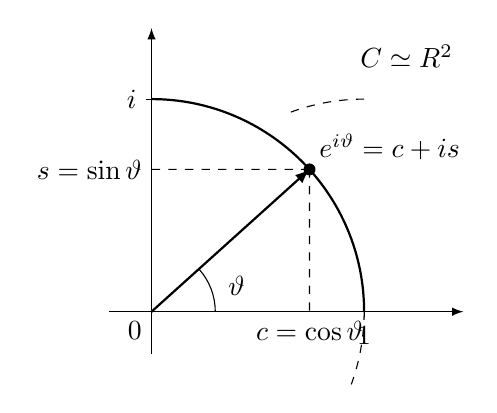
\begin{tikzpicture}[>=latex, scale=1.8]
  % 坐标轴
  \draw[->] (-0.3,0) -- (2.2,0);
  \draw[->] (0,-0.3) -- (0,2.0);
  
  % 原点
  \node[below left] at (0,0) {$0$};
  
  % 单位圆弧 (第 I 象限及两端延展)
  \draw[thick] (1.5,0) arc (0:90:1.5);
  \draw[dashed] (1.5,0) arc (0:-20:1.5);
  \draw[dashed] (1.5,0) ++(90:1.5) arc (90:112:1.5);
  
  % 刻度 1 与 i
  \draw (1.5,-0.04) -- (1.5,0.04) node[below=4pt]{$1$};
  \draw (-0.04,1.5) -- (0.04,1.5) node[left=4pt]{$i$};
  
  % 向量与点 e^{i vartheta}
  \coordinate (Z) at ({1.5*cos(42)}, {1.5*sin(42)});
  \draw[thick, ->] (0,0) -- (Z);
  \fill (Z) circle (1.2pt) node[above right]{$e^{i\vartheta} = c + is$};
  
  % 夹角 vartheta
  \draw (0.45,0) arc (0:42:0.45);
  \node at (0.60,0.18) {$\vartheta$};
  
  % 虚线投影与三角函数值
  \draw[dashed] (Z) -- ({1.5*cos(42)}, 0) node[below]{$c = \cos \vartheta$};
  \draw[dashed] (Z) -- (0, {1.5*sin(42)}) node[left]{$s = \sin \vartheta$};
  
  % 右上角复平面记号
  \node at (1.8, 1.8) {$\mathbb{C} \simeq \mathbb{R}^2$};
\end{tikzpicture}
\end{center}

由于复数的乘法把模相乘并把辐角相加(模 $2\pi$), 且 $e^{i\vartheta}$ 的模为 $1$, 确实可以把 $\mathbb{R}$-线性映射 $\mathbb{C} \longrightarrow \mathbb{C}$, $z \longmapsto e^{i\vartheta} z$, 从而把上述映射 $\varphi \colon \mathbb{R}^2 \longrightarrow \mathbb{R}^2$ 识别为以角度 $\vartheta$ 的旋转.由于 $e^{i\vartheta} = \cos \vartheta + i \sin \vartheta$, 描述矩阵具有形式

\[
R(\vartheta) = \begin{pmatrix} \cos \vartheta & -\sin \vartheta \\ \sin \vartheta & \cos \vartheta \end{pmatrix} \in \mathbb{R}^{2 \times 2}, \qquad 0 \leq \vartheta \leq 2\pi,
\]

并被称为角度 $\vartheta$ 的\emph{旋转矩阵}(\textup{Drehmatrix; R})\index{xuanzhuanjuzhen@旋转矩阵(Drehmatrix; R)}.反过来显然, 每个这样的旋转矩阵在实平面 $\mathbb{R}^2$ 上定义了一个旋转, 从而是一个等距同构.

除旋转之外, $\mathbb{R}^2$ 还有另外的等距同构, 即所谓的反射.$\mathbb{R}$-线性映射 $\varphi \colon \mathbb{R}^2 \longrightarrow \mathbb{R}^2$ 称为一个反射, 如果存在 $\mathbb{R}^2$ 的一个标准正交基 $u_1, u_2$, 使得 $\varphi$ 由

\[
u_1 \longmapsto u_1, \qquad u_2 \longmapsto -u_2
\]

描述.下面的定理~\mtref{thm:7.5.6} 将告诉我们, 旋转和反射是 $\mathbb{R}^2$ 仅有的等距同构.不过我们首先想回到定理~\mtref{thm:7.5.1} 的一般情形, 再作一些推论.

\begin{corollary}\label{cor:7.5.3}
对 $\varphi \in \operatorname{End}_K(V)$, 下列条件等价:
\begin{enumerate}
\item[(i)] $\varphi$ 是一个等距同构;
\item[(ii)] 若 $X$ 是 $V$ 的一个标准正交基, 则 $A_{\varphi, X, X}$ 可逆, 并且成立
\[
(A_{\varphi, X, X})^* = (A_{\varphi, X, X})^{-1};
\]
\item[(iii)] 存在 $V$ 的一个标准正交基 $X$, 使得 $A_{\varphi, X, X}$ 可逆并且成立
\[
(A_{\varphi, X, X})^* = (A_{\varphi, X, X})^{-1}\text{.}
\]
\end{enumerate}
\end{corollary}

\begin{proof}
利用注记~\mtref{rem:7.4.4} 与定理~\mtref{thm:7.5.1} (ii).
\end{proof}

最后容易看出, 推论~\mtref{cor:7.5.3} (ii) 或 (iii) 中的性质 $A^* = A^{-1}$ 也可以用来刻画把 $V$ 的标准正交基变为标准正交基的基变换矩阵.

\begin{theorem}\label{thm:7.5.4}
设 $X$ 是一个标准正交基, $Y$ 是 $V$ 的另一个基.则下列条件等价:
\begin{enumerate}
\item[(i)] $Y$ 是 $V$ 的一个标准正交基;
\item[(ii)] 对基变换矩阵 $A = A_{Y, X}$ 成立 $A^* = A^{-1}$.
\end{enumerate}
\end{theorem}

\begin{proof}
设 $\varphi \colon V \longrightarrow V$ 是把基 $X$ 映到基 $Y$ 的 $K$-线性映射; 此时成立

\[
A_{\varphi, X, X} = A = A_{Y, X}\text{.}
\]

按定理~\mtref{thm:7.5.1} (iv) 或 (v), $Y$ 是一个标准正交基, 当且仅当 $\varphi$ 是一个等距同构, 而按推论~\mtref{cor:7.5.3} 这等价于 $(A_{\varphi, X, X})^* = (A_{\varphi, X, X})^{-1}$, 即等价于 $A^* = A^{-1}$.
\end{proof}

矩阵 $A \in \mathbb{R}^{n \times n}$ 称为正交的, 如果 $\mathbb{R}$-线性映射

\[
\mathbb{R}^n \longrightarrow \mathbb{R}^n, \qquad x \longmapsto A x,
\]

是正交的, 即是一个等距同构.其中借助标准数量积把 $\mathbb{R}^n$ 看作欧几里得向量空间.按推论~\mtref{cor:7.5.3}, 矩阵 $A \in \mathbb{R}^{n \times n}$ 的正交性等价于条件 $A^t = A^{-1}$ 或 $A^t A = E$, 其中 $E \in \mathbb{R}^{n \times n}$ 是单位矩阵.若 $a_1, \ldots, a_n \in \mathbb{R}^n$ 是 $A$ 的列, 则这个条件正是

\[
a_i^t \cdot a_j = \delta_{ij}, \qquad i, j = 1, \ldots, n\text{.}
\]

对 $A$ 的行也可以作相应的考虑.因此矩阵 $A \in \mathbb{R}^{n \times n}$ 正交, 当且仅当其列(或行)组成一个标准正交系, 从而组成 $\mathbb{R}^n$ 的一个标准正交基.

在域 $\mathbb{C}$ 上类似地处理.矩阵 $A \in \mathbb{C}^{n \times n}$ 称为酉的, 如果 $\mathbb{C}$-线性映射

\[
\mathbb{C}^n \longrightarrow \mathbb{C}^n, \qquad x \longmapsto A x,
\]

是酉的, 即是一个等距同构.其中借助标准数量积把 $\mathbb{C}^n$ 看作酉向量空间.按推论~\mtref{cor:7.5.3}, $A \in \mathbb{C}^{n \times n}$ 酉, 当且仅当 $A^* = A^{-1}$ 或 $A^* A = E$ 成立, 而这个条件又等价于 $A$ 的列(或行)组成 $\mathbb{C}^n$ 的一个标准正交基.

由推论~\mtref{cor:7.5.2} 和推论~\mtref{cor:7.5.3} 立即得出, 正交或酉矩阵 $A \in K^{n \times n}$ 组成 $K^{n \times n}$ 中一切可逆矩阵的群 $\mathrm{Gl}(n, K)$ 的一个子群.其中人们把

\[
\mathrm{O}(n) = \bigl\{A \in \mathrm{Gl}(n, \mathbb{R});\; A^t = A^{-1}\bigr\}
\]

称为指标 $n$ 的\emph{正交群}(\textup{orthogonale Gruppe; O(n)})\index{zhengjiaoqun@正交群(orthogonale Gruppe; O(n))}, 把

\[
\mathrm{U}(n) = \bigl\{A \in \mathrm{Gl}(n, \mathbb{C});\; A^* = A^{-1}\bigr\}
\]

称为指标 $n$ 的\emph{酉群}(\textup{unitäre Gruppe; U(n)})\index{youqun@酉群(unitäre Gruppe; U(n))}, 其中可以把 $\mathrm{O}(n)$ 看作 $\mathrm{U}(n)$ 的子群.对 $A \in \mathrm{U}(n)$, $A^* \cdot A$ 是单位矩阵, 所以对每个正交或酉矩阵都得到 $|\det(A)| = 1$.特别地, 可以把

\[
\mathrm{SO}(n) = \bigl\{A \in \mathrm{O}(n);\; \det(A) = 1\bigr\}
\]

看作正交群的子群; 人们把这个群称为\emph{特殊正交群}(\textup{spezielle orthogonale Gruppe; SO(n)})\index{teshuzhengjiaoqun@特殊正交群(spezielle orthogonale Gruppe; SO(n))}.

我们想在 $n = 2$ 的情形更精确地描述正交群 $\mathrm{O}(2)$.上面已经证明, 旋转矩阵

\[
R(\vartheta) = \begin{pmatrix} \cos \vartheta & -\sin \vartheta \\ \sin \vartheta & \cos \vartheta \end{pmatrix} \in \mathbb{R}^{2 \times 2}, \qquad 0 \leq \vartheta < 2\pi,
\]

给出 $\mathbb{R}^2$ 的等距同构, 从而属于 $\mathrm{O}(2)$, 甚至属于子群 $\mathrm{SO}(2)$, 因为总有 $\det(R(\vartheta)) = 1$.我们首先想证明 $\mathrm{SO}(2)$ 不含另外的矩阵.为此考察一个矩阵

\[
A = \begin{pmatrix} \alpha_{11} & \alpha_{12} \\ \alpha_{21} & \alpha_{22} \end{pmatrix} \in \mathrm{O}(2)\text{.}
\]

则关系

\[
\begin{pmatrix} 1 & 0 \\ 0 & 1 \end{pmatrix} = A^t \cdot A = \begin{pmatrix} \alpha_{11}^2 + \alpha_{21}^2 & \alpha_{11}\alpha_{12} + \alpha_{21}\alpha_{22} \\ \alpha_{12}\alpha_{11} + \alpha_{22}\alpha_{21} & \alpha_{12}^2 + \alpha_{22}^2 \end{pmatrix}
\]

给出方程组

\[
\begin{array}{c}
\alpha_{11}^2 + \alpha_{21}^2 = 1, \\
\alpha_{12}^2 + \alpha_{22}^2 = 1, \\
\alpha_{11}\alpha_{12} + \alpha_{21}\alpha_{22} = 0\text{.}
\end{array}
\]

复数

\[
\alpha_{11} + i\alpha_{21}, \qquad \alpha_{22} + i\alpha_{12}
\]

因此绝对值为 $1$.它们的乘积亦然, 于是有

\[
\begin{array}{c}
\bigl(\alpha_{11} + i\alpha_{21}\bigr) \cdot \bigl(\alpha_{22} + i\alpha_{12}\bigr) = \bigl(\alpha_{11}\alpha_{22} - \alpha_{21}\alpha_{12}\bigr) + i\bigl(\alpha_{11}\alpha_{12} + \alpha_{21}\alpha_{22}\bigr) \\
= \alpha_{11}\alpha_{22} - \alpha_{21}\alpha_{12} \\
= \det(A) = \pm 1 \in \mathbb{R}\text{.}
\end{array}
\]

现在利用对绝对值 $1$ 的复数 $z$ 恒有 $z\overline{z} = 1$, 于是在 $\det(A) = 1$ 的情形, 即在 $A \in \mathrm{SO}(2)$ 的情形, 得到

\[
\alpha_{22} + i\alpha_{12} = \overline{\alpha_{11} + i\alpha_{21}} = \alpha_{11} - i\alpha_{21},
\]

从而

\[
\alpha_{22} = \alpha_{11}, \qquad \alpha_{12} = -\alpha_{21}\text{.}
\]

现在我们利用分析中的事实: 由于 $\alpha_{11}^2 + \alpha_{21}^2 = 1$, 存在唯一的角度 $\vartheta$, $0 \leq \vartheta < 2\pi$, 使得

\[
\alpha_{11} + i\alpha_{21} = \cos \vartheta + i \sin \vartheta = e^{i\vartheta},
\]

即

\[
A = \begin{pmatrix} \alpha_{11} & -\alpha_{21} \\ \alpha_{21} & \alpha_{11} \end{pmatrix} = \begin{pmatrix} \cos \vartheta & -\sin \vartheta \\ \sin \vartheta & \cos \vartheta \end{pmatrix} = R(\vartheta)\text{.}
\]

这意味着 $A$ 描述了围绕零点以角度 $\vartheta$ 的旋转.

旋转 $R(\vartheta)$ 的特征多项式计算为

\[
\chi_{R(\vartheta)} = T^2 - 2(\cos \vartheta) T + 1 = (T - e^{i\vartheta})(T - e^{-i\vartheta}),
\]

所以只有在 $\sin \vartheta = 0$, 即 $\vartheta \in \{0, \pi\}$ 的情形才有实零点.于是得到:

\begin{theorem}\label{thm:7.5.5}
$\mathrm{SO}(2)$ 由一切在 $\mathbb{R}^2$ 中引起围绕零点旋转的实 $(2 \times 2)$-矩阵组成, 即

\[
\mathrm{SO}(2) = \bigl\{R(\vartheta);\; 0 \leq \vartheta < 2\pi\bigr\}\text{.}
\]
\end{theorem}

除平凡情形 $R(0) = \mathrm{id}$ 与 $R(\pi) = -\mathrm{id}$ 外, 矩阵 $R(\vartheta)$ 没有实特征值, 从而也不可对角化.

对满足 $\det(A) = -1$ 的矩阵 $A = (\alpha_{ij})_{i, j = 1, 2} \in \mathrm{O}(2)$, 上面的计算以相应方式给出恒等式

\[
\alpha_{22} + i\alpha_{12} = -\overline{(\alpha_{11} + i\alpha_{21})} = -\alpha_{11} + i\alpha_{21},
\]

即

\[
\alpha_{22} = -\alpha_{11}, \qquad \alpha_{12} = \alpha_{21},
\]

所以在这个情形也存在唯一的角度 $\vartheta$, $0 \leq \vartheta < 2\pi$, 使得

\[
A = \begin{pmatrix} \cos \vartheta & \sin \vartheta \\ \sin \vartheta & -\cos \vartheta \end{pmatrix}\text{.}
\]

自然, 这个类型的所有矩阵 $A$ 都属于 $\mathrm{O}(2)$.这样的矩阵的特征多项式计算为 $\chi_A = T^2 - 1$, 所以 $A$ 具有实特征值 $1$ 与 $-1$, 从而可对角化.方程 $A^t = A^{-1}$ 表明, $A$ 描述 $\mathbb{R}^2$ 的一个\emph{正规自同态}(\textup{normaler Endomorphismus})\index{zhengguizitongtai@正规自同态(normaler Endomorphismus)}.按定理~\mtref{thm:7.4.8}, 此时 $\mathbb{R}^2$ 中存在一个由 $A$ 的特征向量组成的标准正交基, 并且看出 $A$ 是一个反射.于是得到:

\begin{theorem}\label{thm:7.5.6}
$\mathrm{O}(2)$ 由一切在 $\mathbb{R}^2$ 中引起旋转或反射的实 $(2 \times 2)$-矩阵组成.更确切地说, 成立

\[
\mathrm{O}(2) = \left\{\begin{pmatrix} \cos \vartheta & -\sin \vartheta \\ \sin \vartheta & \cos \vartheta \end{pmatrix}, \begin{pmatrix} \cos \vartheta & \sin \vartheta \\ \sin \vartheta & -\cos \vartheta \end{pmatrix} \in \mathbb{R}^{2 \times 2};\; 0 \leq \vartheta < 2\pi\right\}\text{.}
\]
\end{theorem}

群 $\mathrm{O}(2)$ 与 $\mathrm{SO}(2)$ 的结构由此完全清楚了.还应该指出(并可以用初等计算验证), $\mathrm{SO}(2)$ 是交换的, 而 $\mathrm{O}(2)$ 不是.

下面我们想推导欧几里得和酉向量空间中一般类型\emph{等距同构的标准形}(\textup{Normalform für orthogonale und unitäre Abbildungen})\index{dengjutonggoudebiaozhunxing@等距同构的标准形(Normalform für orthogonale und unitäre Abbildungen)}.由定理~\mtref{thm:7.5.1} (ii) 特别推出, 每个等距同构都是正规的.相应地, 至少在复数域 $\mathbb{C}$ 上可以应用谱定理~\mtref{thm:7.4.8}.

\begin{theorem}\label{thm:7.5.7}
设 $\varphi \in \operatorname{End}_{\mathbb{C}}(V)$ 是有限维酉 $\mathbb{C}$-向量空间 $V$ 的自同态.则下列条件等价:
\begin{enumerate}
\item[(i)] $\varphi$ 是一个等距同构;
\item[(ii)] 对 $\varphi$ 的每个特征值 $\lambda$ 成立 $|\lambda| = 1$, 并且存在关于 $\varphi$ 的特征向量组成 $V$ 的一个标准正交基.
\end{enumerate}
\end{theorem}

\begin{proof}
首先设 (i) 成立, 即 $\varphi$ 是一个等距同构.则 $\varphi$ 作为保长映射只能有绝对值为 $1$ 的特征值.此外, 由于 $\mathbb{C}$ 代数闭, 特征多项式 $\chi_\varphi$ 完全分裂为一次因式.而且 $\varphi$ 正规.于是由定理~\mtref{thm:7.4.8} 推出存在 $V$ 的一个由关于 $\varphi$ 的特征向量组成的标准正交基 $X$, 即 (ii) 成立.

反之, 若 $X$ 是 $V$ 的一个由关于 $\varphi$ 的特征向量组成的标准正交基, 且所有特征值的绝对值都是 $1$, 则 $X$ 被 $\varphi$ 显然又变换为一个标准正交基.按定理~\mtref{thm:7.5.1}, $\varphi$ 从而是一个等距同构.
\end{proof}

特别地, 有限维酉向量空间的每个等距同构都可对角化.不过对欧几里得向量空间不能指望相应的结果, 正如 $\mathbb{R}^2$ 中围绕零点的旋转的例子所表明的.这里的情形要更复杂一些.

\begin{theorem}\label{thm:7.5.8}
设 $\varphi \in \operatorname{End}_{\mathbb{R}}(V)$ 是有限维欧几里得 $\mathbb{R}$-向量空间 $V$ 的自同态.则下列条件等价:
\begin{enumerate}
\item[(i)] $\varphi$ 是一个等距同构;
\item[(ii)] 存在 $V$ 的一个标准正交基 $X$, 使得 $\varphi$ 关于 $X$ 由一个如下类型的矩阵描述:
\[
A = A_{\varphi, X, X} = \operatorname{Diag}\bigl(E_k, -E_\ell, R(\vartheta_1), \ldots, R(\vartheta_m)\bigr)
\]
\[
= \begin{pmatrix}
E_k & & & & & \\
& -E_\ell & & & & \\
& & R(\vartheta_1) & & & \\
& & & \ddots & & \\
& & & & \ddots & \\
& & & & & R(\vartheta_m)
\end{pmatrix}
\]
其中 $E_k \in \mathbb{R}^{k \times k}$(或 $E_\ell \in \mathbb{R}^{\ell \times \ell}$)是行数和列数为 $k$(或 $\ell$)的单位矩阵, 而 $R(\vartheta_1), \ldots, R(\vartheta_m) \in \mathbb{R}^{2 \times 2}$ 是某个角度 $0 < \vartheta_1 \leq \vartheta_2 \leq \cdots \leq \vartheta_m < \pi$ 的旋转矩阵.
\end{enumerate}

若 $\varphi$ 是一个等距同构, 则 (ii) 中的标准形连同数 $k$, $\ell$, $m$ 与角度 $\vartheta_1, \ldots, \vartheta_m$ 被 $\varphi$ 唯一确定, 并且成立

\[
\chi_\varphi = (T - 1)^k (T + 1)^\ell \prod_{j = 1}^{m} (T - e^{i\vartheta_j})(T - e^{-i\vartheta_j})\text{.}
\]
\end{theorem}

\begin{proof}
首先设 $\varphi$ 是一个等距同构.为推导 (ii) 中断言的标准形, 我们按 $V$ 的维数 $n$ 作归纳.在 $n = 0$ 的情形没有要证的, 设 $n > 0$.我们断言, 此时 $V$ 含有维数为 $1$ 或 $2$ 的 $\varphi$-不可分解线性子空间 $U$.由大定理~\mtref{bigthm:6.5.6} 得出, $V$ 至少有一个 $\varphi$-不变子空间 $U'$, 它在 $\varphi$ 下作为 $\mathbb{R}[T]$-模同构于一个商 $\mathbb{R}[T]/(p^c)$; 其中 $p \in \mathbb{R}[T]$ 是一个素多项式, $c \geq 1$ 是一个幂指数.用 $p^{c-1}$ 相乘定义了一个 $\mathbb{R}[T]$-模同构 $\mathbb{R}[T] \xrightarrow{\sim} p^{c-1}\mathbb{R}[T]$, 并且通过取商定义了一个 $\mathbb{R}[T]$-模同构 $\mathbb{R}[T]/p\mathbb{R}[T] \xrightarrow{\sim} p^{c-1}\mathbb{R}[T]/p^c\mathbb{R}[T]$, 其中可以把 $p^{c-1}\mathbb{R}[T]/p^c\mathbb{R}[T]$ 看作 $\mathbb{R}[T]/(p^c)$ 的 $\mathbb{R}[T]$-子模.于是由注记~\mtref{rem:6.5.2} (i), $U'$ 从而特别地 $V$ 含有一个 $\varphi$-不变的线性子空间 $U$, 它作为 $\mathbb{R}[T]$-模同构于 $\mathbb{R}[T]/(p)$, 从而按定理~\mtref{thm:6.5.4} 或推论~\mtref{cor:6.5.7} 是 $\varphi$-不可分解的, 并且按引理~\mtref{lem:6.5.5} 具有维数 $\operatorname{grad} p$.而 $\mathbb{R}[T]$ 中的素多项式次数为 $1$ 或 $2$, 参见 \ref{sec:5.3} 节习题 3, 于是我们认识到 $U \subset V$ 是维数为 $1$ 或 $2$ 的不可分解 $\varphi$-不变线性子空间.

现在我们考察分解 $V = U \oplus U^{\perp}$, 参见推论~\mtref{cor:7.2.8}, 并且证明, 与 $U$ 一起, 正交补 $U^{\perp}$ 也是 $V$ 的 $\varphi$-不变子空间.为此我们首先注意到, $\varphi$ 作为同构诱导了一个线性映射 $\varphi|_{U} \colon U \longrightarrow U$, 它至少是单射, 但随后由推论~\mtref{cor:2.1.11} 甚至是双射, 从而满足 $\varphi^{-1}(U) = U$.现在设 $y \in U^{\perp}$.则对一切 $x \in U$ 成立

\[
\bigl\langle x, \varphi(y) \bigr\rangle = \bigl\langle \varphi^*(x), y \bigr\rangle = \bigl\langle \varphi^{-1}(x), y \bigr\rangle = 0,
\]

因为正如我们看到的, 与 $x$ 一起 $\varphi^{-1}(x)$ 也属于 $U$.但这意味着 $\varphi(y) \in U^{\perp}$, 于是我们认识到确实 $U^{\perp}$ 是 $V$ 的 $\varphi$-不变子空间.

现在在 $U$ 中选取一个标准正交基 $X'$.在 $\dim_{\mathbb{R}}(U) = 1$ 的情形, $X'$ 只由一个向量组成, 它必然是 $\varphi$ 的特征向量.相应的特征值按定理~\mtref{thm:7.5.1} (iii) 绝对值为 $1$, 即等于 $1$ 或 $-1$.对 $\dim_{\mathbb{R}}(U) = 2$, $X'$ 由两个向量组成, 并且由推论~\mtref{cor:7.5.3} 推出矩阵 $A_{\varphi|_{U}, X', X'}$ 属于 $\mathrm{O}(2)$, 但不可能可对角化, 因为我们曾假定 $U$ 是 $\varphi$-不可分解的.于是由上面关于 $\mathrm{O}(2)$ 中矩阵的描述, 必然有 $A_{\varphi|_{U}, X', X'} = R(\vartheta)$, 其中角度 $\vartheta \neq \pi$, $0 < \vartheta < 2\pi$.必要时通过改变 $X'$ 中向量的顺序(这相当于把角度 $\vartheta$ 换成 $2\pi - \vartheta$), 甚至可以假定 $0 < \vartheta < \pi$.

按归纳假设, $U^{\perp}$ 中存在一个标准正交基 $X''$, 使得 $A_{\varphi|_{U^{\perp}}, X'', X''}$ 具有 (ii) 中描述的形式.于是可以把 $X'$ 与 $X''$ 合成 $V$ 的一个标准正交基 $X$, 并且经过对 $X$ 的基向量适当重新编号, 矩阵 $A_{\varphi, X, X}$ 具有所求的形式.蕴含关系 (i) $\Longrightarrow$ (ii) 得证.反之显然, (ii) 类型的每个矩阵都是正交的, 故在此情形 $\varphi$ 是一个等距同构.

为证唯一性断言, 只需注意: 对等距同构 $\varphi$, 一个如 (ii) 中的描述矩阵 $A$ 的特征多项式计算为

\[
\chi_\varphi = \chi_A = (T - 1)^k (T + 1)^\ell \prod_{j = 1}^{m} (T - e^{i\vartheta_j})(T - e^{-i\vartheta_j})
\]

于是 $\chi_\varphi$ 首先确定 $A$ 中的数 $k$, $\ell$ 与 $m$.由于在成对的复共轭零点 $e^{i\vartheta_j}, e^{-i\vartheta_j}$ 中实部 $\cos \vartheta_j$ 各自相等, 而这个实部唯一确定 $0 < \vartheta_j < \pi$ 范围内的角度, 所以矩阵 $A$ 的整体形状由多项式 $\chi_\varphi$ 确定.
\end{proof}

\aufgaben

除非另外规定, $V$ 恒为有限维欧几里得或酉 $K$-向量空间.

\medskip
\noindent\textbf{习题 1.} 证明: 对 $x, y \in V$, 存在等距同构 $\varphi \in \operatorname{End}_K(V)$ 使得 $\varphi(x) = y$, 当且仅当 $|x| = |y|$ 成立.

\medskip
\noindent\textbf{习题 2.} 对带角度 $0 \leq \vartheta_1 < \vartheta_2 < 2\pi$ 的旋转矩阵 $R(\vartheta_1), R(\vartheta_2) \in \mathbb{R}^{2 \times 2}$ 证明: 它们相似, 当且仅当 $\vartheta_1 + \vartheta_2 = 2\pi$ 成立.(AT 368)

\medskip
\noindent\textbf{习题 3.} 设 $e_1, \ldots, e_n \in \mathbb{R}^n$ 是典范单位向量, 理解为列向量.矩阵 $A \in \mathbb{R}^{n \times n}$ 称为置换矩阵, 如果存在置换 $\pi \in \mathfrak{S}_n$ 使得 $A = E_\pi := (e_{\pi(1)}, \ldots, e_{\pi(n)})$.证明:
\begin{enumerate}
\item[(i)] 每个置换矩阵可逆, 且典范映射 $\sigma \colon \mathfrak{S}_n \longrightarrow \mathrm{Gl}(n, \mathbb{R})$, $\pi \longmapsto E_\pi$ 定义了单射的群同态;
\item[(ii)] 对一切 $\pi \in \mathfrak{S}_n$ 成立 $E_\pi \in \mathrm{O}(n)$;
\item[(iii)] 设 $A = (\alpha_{ij}) \in \mathrm{O}(n)$ 是带系数 $\alpha_{ij} \geq 0$ 的\emph{正交矩阵}(\textup{orthogonale Matrix})\index{zhengjiaojuzhen@正交矩阵(orthogonale Matrix)}.则 $A$ 已经是一个置换矩阵.
\end{enumerate}

\medskip
\noindent\textbf{习题 4.} 设 $A = (\alpha_{ij}) \in \mathrm{O}(n)$ 是下三角形正交矩阵, 即对 $i < j$ 成立 $\alpha_{ij} = 0$.证明: $A$ 甚至是对角矩阵.对矩阵 $A \in \mathrm{U}(n)$ 相应的断言也成立吗? (AT 369)

\medskip
\noindent\textbf{习题 5.} 设 $A, B \in \mathbb{C}^{n \times n}$ 是酉矩阵.证明: $A$ 与 $B$ 相似, 当且仅当它们酉相似, 即存在酉矩阵 $S \in \mathbb{C}^{n \times n}$ 使得 $B = S^{-1} A S$.在域 $K = \mathbb{R}$ 上以"正交"代替"酉"相应的断言也成立吗?

\section{自伴随映射}\index{zibansuide@自伴随的(selbstadjungiert)}\label{sec:7.6}

仍设 $V$ 是带数量积 $\varPhi \colon V \times V \longrightarrow K$ 的有限维 $K$-向量空间, 即一个欧几里得或酉向量空间.

\begin{definition}\label{def:7.6.1}
自同态 $\varphi \in \operatorname{End}_K(V)$ 称为\emph{自伴随的}(\textup{selbstadjungiert})\index{zibansuide@自伴随的(selbstadjungiert)}, 如果成立 $\varphi^* = \varphi$.

矩阵 $A \in K^{n \times n}$ 称为对称的(在 $K = \mathbb{R}$ 的情形)或埃尔米特的(在 $K = \mathbb{C}$ 的情形), 如果成立 $A^* = A$.
\end{definition}

对任意自同态 $\varphi \colon V \longrightarrow V$, 复合 $\varphi \circ \varphi^*$ 是自伴随的, 正如等式

\[
\bigl\langle \varphi \circ \varphi^*(x), y \bigr\rangle = \bigl\langle \varphi^*(x), \varphi^*(y) \bigr\rangle = \bigl\langle x, \varphi \circ \varphi^*(y) \bigr\rangle, \qquad x, y \in V,
\]

所表明的.相应地, 对每个矩阵 $A \in K^{n \times n}$, 乘积 $A A^*$ 是对称或埃尔米特的.此外, $V$ 的每个自伴随自同态都特别地是正规的.借助注记~\mtref{rem:7.4.4} 得到下列自伴随自同态的刻画:

\begin{remark}\label{rem:7.6.2}
设 $X$ 是 $V$ 的一个标准正交基.则对 $\varphi \in \operatorname{End}_K(V)$, 下列条件等价:
\begin{enumerate}
\item[(i)] $\varphi$ 自伴随;
\item[(ii)] $(A_{\varphi, X, X})^* = A_{\varphi, X, X}$, 即 $A_{\varphi, X, X}$ 对称或埃尔米特.
\end{enumerate}
\end{remark}

基于我们对正规自同态的研究, 现在可以作出如下重要观察:

\begin{theorem}\label{thm:7.6.3}
设 $\varphi \in \operatorname{End}_K(V)$ 自伴随.则特征多项式 $\chi_\varphi$ 具有实系数, 并在 $\mathbb{R}[T]$ 中完全分裂为一次因式.特别地, $\varphi$ 只有实特征值.
\end{theorem}

\begin{proof}
首先设 $K = \mathbb{C}$.由推论~\mtref{cor:7.4.7} 得 $\lambda = \overline{\lambda}$, 从而对 $\varphi$ 的一切特征值 $\lambda$ 或 $\chi_\varphi$ 的一切零点成立 $\lambda \in \mathbb{R}$.利用 $\mathbb{C}$ 代数闭这一事实, 我们看到 $\chi_\varphi$ 完全分裂为一次因式, 并且这些因式都是实的.特别地 $\chi_\varphi$ 是一个实多项式.

在 $K = \mathbb{R}$ 的情形选取 $V$ 的一个标准正交基 $X$ 并考察矩阵 $A = A_{\varphi, X, X}$, 其中此时成立 $A^* = A^t = A$; 参见注记~\mtref{rem:7.4.4}.现在把以 $n = \dim_{\mathbb{R}} V$ 的 $\mathbb{C}^n$ 在标准数量积下看作酉向量空间, 则 $A$ 作为对称实矩阵特别地也定义了自伴随自同态

\[
\mathbb{C}^n \longrightarrow \mathbb{C}^n, \qquad x \longmapsto A x,
\]

我们可以像上面那样推出, 相应的特征多项式即 $\chi_A$ 完全分裂为实一次因式.但由于 $\chi_A$ 与 $\chi_\varphi$ 一致, 我们得证.
\end{proof}

因此对自伴随自同态, 我们可以把正规自同态的谱定理~\mtref{thm:7.4.8} 强化为:

\begin{corollary}\label{cor:7.6.4}
对自同态 $\varphi \in \operatorname{End}_K(V)$, 下列条件等价:
\begin{enumerate}
\item[(i)] $\varphi$ 自伴随;
\item[(ii)] $\varphi$ 的所有特征值都是实的, 并且 $V$ 有一个由关于 $\varphi$ 的特征向量组成的标准正交基;
\item[(iii)] 在 $V$ 中存在一个标准正交基 $X$, 使得 $A_{\varphi, X, X}$ 是一个实对角矩阵.
\end{enumerate}
\end{corollary}

\begin{proof}
首先设条件 (i) 成立, 即 $\varphi$ 自伴随.则按定理~\mtref{thm:7.6.3}, 特征多项式 $\chi_\varphi$ 具有实系数并在 $\mathbb{R}$ 上完全分裂为一次因式; 因此所有特征值都是实的.由于 $\varphi$ 特别地正规, 按定理~\mtref{thm:7.4.8} 存在 $V$ 的一个由关于 $\varphi$ 的特征向量组成的标准正交基 $X$, 即条件 (ii) 满足.此外由 (ii) 推出矩阵 $A_{\varphi, X, X}$ 具有对角形式, 其中对角线上的正是 $\varphi$ 的特征值.于是 $A_{\varphi, X, X}$ 是一个实对角矩阵, 正如 (iii) 所断言的.

最后, 若存在 $V$ 的一个标准正交基 $X$, 使得 $A_{\varphi, X, X}$ 是一个实对角矩阵, 则成立

\[
(A_{\varphi, X, X})^* = A_{\varphi, X, X},
\]

并由注记~\mtref{rem:7.4.4} 得 $A_{\varphi^*, X, X} = A_{\varphi, X, X}$, 即 $\varphi^* = \varphi$.条件 (iii) 因此蕴含 (i).
\end{proof}

由于可以把满足 $A = A^*$ 的矩阵 $A \in K^{n \times n}$ 总是解释为 $K^n$(配备标准数量积)的自伴随自同态, 作为直接推论得到:

\begin{corollary}\label{cor:7.6.5}
设 $A \in K^{n \times n}$ 是满足条件 $A^* = A$ 的矩阵, 即一个对称或埃尔米特矩阵.则 $A$ 相似于一个实对角矩阵.特别地成立 $\chi_A \in \mathbb{R}[T]$, 并且这个多项式在 $\mathbb{R}[T]$ 中完全分裂为一次因式.
\end{corollary}

在特殊情形 $K = \mathbb{R}$, 对称矩阵 $A \in \mathbb{R}^{n \times n}$ 从而总是可对角化的, 因此(对 $n \geq 1$)至少有一个(实)特征值.

我们在推论~\mtref{cor:7.6.5} 中还没有利用, 在对称或埃尔米特矩阵 $A$ 与相应的实对角矩阵之间传递相似性的基变换矩阵, 按推论~\mtref{cor:7.6.4} 的构造描述的是标准正交基之间的基变换, 从而按定理~\mtref{thm:7.5.4} 是正交或酉的.我们想利用这一点, 并由此得到所谓的主轴变换定理, 我们将推导它的两个不同版本.\index{zhuzhoubianhuan@主轴变换(Hauptachsentransformation)}

\begin{bigtheorem}\label{bigthm:7.6.6}
设 $A \in K^{n \times n}$ 是满足 $A^* = A$ 的矩阵.则存在正交或酉矩阵 $S \in \mathrm{Gl}(n, K)$, 使得

\[
D = S^{-1} A S = S^* A S = (\overline{S})^t A \overline{\overline{S}}
\]

是一个实对角矩阵.其中与 $S$ 一起, $\overline{S} \in \mathrm{Gl}(n, K)$ 也是正交或酉的, 而 $D$ 的对角线元素恰是 $A$ 的特征值.
\end{bigtheorem}

方程 $D = S^{-1} A S$ 表明, $A$ 作为(自伴随)线性映射 $\mathbb{K}^n \longrightarrow \mathbb{K}^n$ 可以借助由 $S$ 给出的基变换化为对角形.相应地, $D = (\overline{S})^t A \overline{\overline{S}}$ 意味着, 由 $A$ 给出的 sBF 或 HF 可以借助由 $\overline{S}$ 给出的基变换化为对角形.

\begin{bigtheorem}\label{bigthm:7.6.7}
设 $V$ 是带数量积 $\varPhi$ 的欧几里得或酉向量空间, 并且设 $\Psi \colon V \times V \longrightarrow K$ 是 $V$ 上任意 sBF 或 HF.则存在 $V$ 的一个标准正交基 $X$, 使得矩阵 $A_{\varPsi, X}$ 是一个实对角矩阵.
\end{bigtheorem}

\begin{proof}[定理~\mtref{bigthm:7.6.6} 的证明]
我们把 $\mathbb{K}^n$ 连同标准数量积看作欧几里得或酉向量空间.则线性映射

\[
\varphi \colon \mathbb{K}^n \longrightarrow \mathbb{K}^n, \qquad x \longmapsto A x,
\]

自伴随, 因为成立 $A^* = A$; 参见注记~\mtref{rem:7.6.2}.按推论~\mtref{cor:7.6.4}, 因此存在 $\mathbb{K}^n$ 的一个标准正交基 $X$, 使得描述矩阵 $D = A_{\varphi, X, X}$ 是一个实对角矩阵.若 $S = A_{X, E} \in \mathrm{Gl}(n, K)$ 是 $X$ 与 $\mathbb{K}^n$ 的典范基 $E$ 之间的基变换矩阵, 则按推论~\mtref{cor:3.4.5} 得到

\[
D = S^{-1} \cdot A \cdot S\text{.}
\]

由于 $S$ 描述两个标准正交基之间的基变换, 按定理~\mtref{thm:7.5.4}, $S$ 正交或酉, 并成立 $S^* = S^{-1}$.通过取共轭得到 $\overline{S}^* = (\overline{S})^{-1}$, 即 $\overline{S}$ 也是正交或酉的.
\end{proof}

\begin{proof}[定理~\mtref{bigthm:7.6.7} 的证明]
我们从 $V$ 的任意一个标准正交基 $X$ 出发; 参见推论~\mtref{cor:7.2.6}.对属于 $\Psi$ 的矩阵, 按推论~\mtref{cor:7.3.4} 成立 $A_{\varPsi, X} = A_{\varPsi, X}^*$, 并且正如我们在定理~\mtref{bigthm:7.6.6} 中看到的, 存在正交或酉矩阵 $S \in \mathrm{Gl}(n, K)$, 使得 $D = S^t \cdot A_{\varPsi, X} \cdot \overline{S}$ 是一个实对角矩阵.我们可以把 $S$ 看作带 $V$ 的新基 $Y$ 的 $A_{Y, X}$ 型基变换矩阵.按定理~\mtref{thm:7.5.4}, $Y$ 又是一个标准正交基, 并且成立

\[
A_{\varPsi, Y} = S^t \cdot A_{\varPsi, X} \cdot \overline{S} = D,
\]

其中可运用定理~\mtref{thm:7.3.5}.于是 $Y$ 代替 $X$ 满足断言.
\end{proof}

为了阐明主轴变换的几何意义, 例如考察 $\mathbb{R}^2$ 中由方程

\[
41 x_1^2 - 24 x_1 x_2 + 34 x_2^2 = 25
\]

给出的曲线 $C$.以 $x = (x_1, x_2)^t$ 以及

\[
A = \begin{pmatrix} 41 & -12 \\ -12 & 34 \end{pmatrix}
\]

则 $C$ 也可以用方程

\[
x^t \cdot A \cdot x = 25
\]

描述.现在我们运用定理~\mtref{bigthm:7.6.6}, 则存在正交矩阵 $S \in \mathrm{O}(2)$, 使得

\[
D = S^t A S = S^{-1} A S
\]

是一个实对角矩阵, 其中 $D$ 的对角线上正是 $A$ 的特征值.由于 $A$ 的特征多项式具有形式

\[
\chi_A = (T - 25)(T - 50),
\]

我们可以取例如

\[
S^t A S = S^{-1} A S = \begin{pmatrix} 25 & 0 \\ 0 & 50 \end{pmatrix}\text{.}
\]

若 $X = E$ 是 $\mathbb{R}^2$ 的典范基, 则可以把 $S$ 看作带新基 $Y$ 的 $A_{Y, X}$ 型基变换矩阵, 其中按定理~\mtref{thm:7.5.4}, $Y$ 又是一个标准正交基.于是按注记~\mtref{rem:3.4.3} 成立关系

\[
\binom{x_1}{x_2} = S \cdot \binom{y_1}{y_2}
\]

介于关于 $X$ 的坐标 $x_1, x_2$ 与关于 $Y$ 的坐标 $y_1, y_2$ 之间, 所以曲线 $C$ 在新坐标下由方程

\[
25 y_1^2 + 50 y_2^2 = 25
\]

即由

\[
y_1^2 + 2 y_2^2 = 1
\]

描述.特别地我们看到, 这是一个椭圆.此时方程中不再出现交叉项, 这意味着人们已经关于 $C$ 的"主轴"来描述 $C$ 了.

\begin{center}
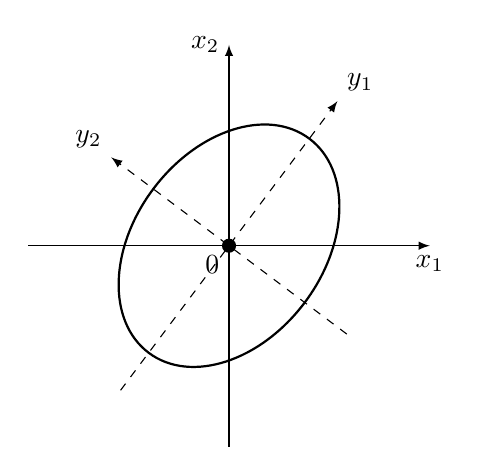
\begin{tikzpicture}[>=latex, scale=1.7]
  \draw[->] (-1.5,0) -- (1.5,0) node[below]{$x_1$};
  \draw[->] (0,-1.5) -- (0,1.5) node[left]{$x_2$};
  \fill (0,0) circle (1.5pt) node[below left]{$0$};
  \draw[rotate=53.13, thick] (0,0) ellipse (1 and 0.7071);
  \begin{scope}[rotate=53.13]
    \draw[->, dashed] (-1.35,0) -- (1.35,0) node[above right]{$y_1$};
    \draw[->, dashed] (0,-1.1) -- (0,1.1) node[above left]{$y_2$};
  \end{scope}
\end{tikzpicture}
\end{center}

为更精确地刻画 $C$, 自然应当显式地确定 $C$ 的主轴, 即标准正交基 $Y$ 和相应的变换矩阵 $S = A_{Y, X}$.这可以如下进行.把

\[
\mathbb{R}^2 \longrightarrow \mathbb{R}^2, \qquad x \longmapsto A x,
\]

看作配备标准数量积的 $\mathbb{R}^2$ 的自伴随自同态, 并确定 $\mathbb{R}^2$ 的一个由关于 $A$ 的特征向量组成的标准正交基 $Y$.为此首先求 $A$ 的特征空间的一个基(通过解相应的线性方程组), 然后按 E.~施密特(Schmidt)对基作正交规范化.在我们的情形这非常简单.

\[
(3, 4)^t, \qquad (-4, 3)^t
\]

是分别属于特征值 $25$ 与 $50$ 的特征向量.规范化后得到

\[
\frac{1}{5}(3, 4)^t, \qquad \frac{1}{5}(-4, 3)^t
\]

作为 $\mathbb{R}^2$ 的标准正交基 $Y$, 以及

\[
S = A_{Y, X} = \frac{1}{5} \begin{pmatrix} 3 & -4 \\ 4 & 3 \end{pmatrix}
\]

作为相应的变换矩阵.其中等距同构

\[
\mathbb{R}^2 \longrightarrow \mathbb{R}^2, \qquad x \longmapsto S x,
\]

可以解释为以大约 $53^{\circ}$ 的角度 $\vartheta$ 的旋转 $R(\vartheta)$.

最后我们还想从主轴变换定理作出一些推论.

\begin{corollary}\label{cor:7.6.8}
对有限维 $K$-向量空间 $V$ 上的 sBF 或 HF $\Psi$, 下列条件等价:
\begin{enumerate}
\item[(i)] $\Psi$ 正定;
\item[(ii)] 存在 $V$ 的一个基 $X$, 使得矩阵 $A_{\varPsi, X}$ 只有正特征值.
\end{enumerate}
\end{corollary}

\begin{proof}
若 $\Psi$ 正定, 则存在关于 $\Psi$ 的 $V$ 的一个标准正交基 $X$.相应的矩阵 $A_{\varPsi, X}$ 此时是单位矩阵.

反之, 设 $X$ 是 $V$ 的一个基, 使得矩阵 $A_{\varPsi, X}$ 只有正特征值.按推论~\mtref{cor:7.3.4} 成立 $A_{\varPsi, X}^* = A_{\varPsi, X}$.由定理~\mtref{bigthm:7.6.6} 于是存在矩阵 $S \in \mathrm{Gl}(n, K)$ 且 $S^* = S^{-1}$, 使得

\[
(\overline{S})^t \cdot A_{\varPsi, X} \cdot \overline{\overline{S}} = S^{-1} A_{\varPsi, X} \cdot S = D
\]

是一个实对角矩阵.其中 $D$ 的对角线元素恰是 $A_{\varPsi, X}$ 的特征值, 从而大于 $0$.若现在把 $\overline{S}$ 解释为带 $V$ 的新基 $Y$ 的 $A_{Y, X}$ 型基变换矩阵, 则成立 $A_{\varPsi, Y} = D$, 并且看出 $\Psi$ 正定.
\end{proof}

\begin{corollary}[Sylvester \emph{惯性定理}\index{guanxingdingli@惯性定理(Sylvester'scher Trägheitssatz)}]\label{cor:7.6.9}\index{guanxingdingli@惯性定理(Sylvester'scher Trägheitssatz)}
设 $\Psi$ 是有限维 $K$-向量空间 $V$ 上的 sBF 或 HF.对 $V$ 的一个基 $X$, 设 $k$ 是 $A_{\varPsi, X}$ 的正特征值个数, $\ell$ 是负特征值个数, $m$ 是消失的特征值个数, 均按重数计数.则成立 $k + \ell + m = \dim_K V$, 并且数 $k$, $\ell$, $m$ 由 $\Psi$ 唯一确定, 特别地与 $X$ 的选取无关.

存在 $V$ 的一个基 $X$, 使得矩阵 $A_{\varPsi, X}$ 具有如下对角形式

\[
A_{\varPsi, X} = \operatorname{Diag}\bigl(\underbrace{1, \ldots, 1}_{k}, \underbrace{-1, \ldots, -1}_{\ell}, \underbrace{0, \ldots, 0}_{m}\bigr),
\]

其中对角线上是 $k$ 个 $1$, $\ell$ 个 $-1$ 和 $m$ 个 $0$.
\end{corollary}

\begin{proof}
我们从 $V$ 的一个基 $X = (x_1, \ldots, x_n)$ 出发, 考察矩阵 $A_{\varPsi, X}$ 及相应的数 $k$, $\ell$, $m$.则按定理~\mtref{bigthm:7.6.6} 结合推论~\mtref{cor:7.3.4}, 存在正交或酉矩阵 $S \in \mathrm{Gl}(n, K)$, 使得 $D = S^t A \overline{S}$ 是一个实对角矩阵; $D$ 的对角线元素恰是 $A$ 的特征值.通过把 $S$ 看作基变换矩阵并用相应的新基代替 $X$, 可以假定

\[
\varPsi(x_i, x_j) = \delta_{ij} \alpha_i
\]

其中 $\alpha_i \in \mathbb{R}$, $i, j = 1, \ldots, n$.此外, 在 $\varPsi(x_i, x_i) \neq 0$ 的情形可以把基向量 $x_i$ 乘以 $|\varPsi(x_i, x_i)|^{-1/2}$, 从而假定 $\alpha_i \in \{1, -1, 0\}$.然后把 $x_i$ 重新编号, 使成立

\[
\alpha_i = \left\{ \begin{array}{l l}
1 & \text{对 } i = 1, \ldots, k \\
-1 & \text{对 } i = k + 1, \ldots, k + \ell \\
0 & \text{对 } i = k + \ell + 1, \ldots, k + \ell + m
\end{array} \right.
\]

则矩阵 $A_{\varPsi, X}$ 具有所断言的形状.

还需证明数 $k$, $\ell$, $m$ 与基 $X$ 的选取无关.设 $X_i$, $i = 1, 2$, 是 $V$ 的两个基, 并设 $k_i$, $\ell_i$, $m_i$ 是相应的数, 其中正如我们刚刚看到的, 可以假定矩阵 $A_{\varPsi, X_i}$ 是实对角矩阵.现在设 $V_i^+ \subset V$ 是由一切满足 $\varPsi(x, x) > 0$ 的 $x \in X_i$ 生成的子空间, $V_i^- \subset V$ 是由一切满足 $\varPsi(x, x) < 0$ 的 $x \in X_i$ 生成的子空间, $V_i^0 \subset V$ 是由一切满足 $\varPsi(x, x) = 0$ 的 $x \in X_i$ 生成的子空间.则对 $i = 1, 2$ 成立

\[
\begin{array}{c}
V = V_i^+ \oplus V_i^- \oplus V_i^0, \\
\dim V_i^+ = k_i, \qquad \dim V_i^- = \ell_i, \qquad \dim V_i^0 = m_i, \\
k_i + \ell_i + m_i = \dim V\text{.}
\end{array}
\]

其中看出

\[
V_1^0 = V_2^0 = \bigl\{x \in V;\; \varPsi(x, y) = 0 \ \text{对一切} \ y \in V\bigr\}
\]

是 $\Psi$ 的"退化空间", 从而成立 $m_1 = m_2$.此外显然有

\[
V_1^+ \cap (V_2^- \oplus V_2^0) = 0,
\]

因为 $\Psi$ 在 $V_1^+$ 上正定而在 $V_2^- \oplus V_2^0$ 上负半定.这意味着

\[
k_1 + \ell_2 + m_2 \leq \dim V
\]

并由 $k_2 + \ell_2 + m_2 = \dim V$ 得到 $k_1 \leq k_2$, 再由对称性理由得 $k_1 = k_2$.于是有

\[
\ell_1 = \dim V - k_i - m_i = \ell_2, \qquad i = 1, 2,
\]

从而得证.
\end{proof}

\aufgaben

除非另外规定, $V$ 恒为有限维欧几里得或酉 $K$-向量空间.

\medskip
\noindent\textbf{习题 1.} 设 $\varphi \in \operatorname{End}_K(V)$ 自伴随.证明: $\varphi$ 恰好具有全部正实特征值, 当且仅当对一切 $x \in V - \{0\}$ 成立 $\langle \varphi(x), x \rangle > 0$.(AT 370)

\medskip
\noindent\textbf{习题 2.} 对正规自同态 $\varphi \in \operatorname{End}_K(V)$ 证明: $\varphi \circ \varphi^*$ 的全部特征值都是实数 $\geq 0$.

\medskip
\noindent\textbf{习题 3.} 对 $A \in \mathbb{R}^{n \times n}$ 证明: $A$ 对称, 当且仅当存在矩阵 $S \in \mathbb{C}^{n \times n}$ 使得 $A = S^t S$.(AT 370)

\medskip
\noindent\textbf{习题 4.} 设 $A \in K^{n \times n}$ 对称或埃尔米特.证明: $A$ 在 $K^n$ 上定义正半定的半双线性形式, 当且仅当 $A$ 具有 $S^* S$ 的形式, 其中 $S \in K^{n \times n}$ 是某个矩阵.

\medskip
\noindent\textbf{习题 5.} 证明: 两个对称或埃尔米特矩阵 $A, B \in K^{n \times n}$ 相似, 当且仅当存在正交或酉矩阵 $S \in \mathrm{Gl}(n, K)$ 使得 $B = S^t A \overline{S}$.
